%!TEX program = pdflatex

\documentclass[acmsmall,nonacm,anonymous,review,screen]{acmart}

\usepackage[utf8]{inputenc}
\usepackage[T1]{fontenc}
\usepackage{microtype}

% ---------- My Packages ----------

\usepackage[commandnameprefix=ifneeded,commentmarkup=footnote]{changes}
\usepackage{xspace}
\usepackage{booktabs}
\usepackage{multirow}
\usepackage{enumitem}
%\setlist{topsep=5pt}
\usepackage{makecell}
\usepackage{tikz}
\usetikzlibrary{shapes.misc}
\usetikzlibrary{decorations.pathreplacing}
\usetikzlibrary{tikzmark}
\usetikzlibrary{positioning}
\usepackage{adjustbox}
\usepackage[dvipsnames,table]{xcolor}
\usepackage{wrapfig}
\usepackage{listings}
\usepackage{lipsum}
\usepackage{mathpartir}
\usepackage{algorithm}
\usepackage{algpseudocode}
\renewcommand{\algorithmicrequire}{\textbf{Input:}}
\renewcommand{\algorithmicensure}{\textbf{Output:}}
\algtext*{EndProcedure}
\algtext*{EndIf}
\algtext*{EndFor}
\algtext*{EndWhile}
\usepackage{caption}
\usepackage{subcaption}
\captionsetup[algorithm]{font=footnotesize}

% ---------- My Commands ----------

\DeclareRobustCommand{\circled}[1]{
    \tikz[baseline=(char.base)]{
        \node[shape=circle, draw, inner sep=0.5pt] (char) {#1};
    }
}
\DeclareRobustCommand{\roundbox}[1]{
    \tikz[baseline=(word.base)]{
        \node [rounded rectangle, draw=black, fill=white, inner sep=4pt] (word) {#1};
    }
}

\newcommand{\textred}[1]{\textcolor{BrickRed}{#1}}
\newcommand{\textgreen}[1]{\textcolor{ForestGreen}{#1}}
\newcommand{\textorange}[1]{\textcolor{BurntOrange}{#1}}
\newcommand{\textblue}[1]{\textcolor{Blue}{#1}}
\newcommand{\textpurple}[1]{\textcolor{Purple}{#1}}
\newcommand{\textgray}[1]{\textcolor{Gray}{#1}}

\DeclareRobustCommand{\endparagraph}{\vspace{1.2ex plus 1ex minus 0.2ex}}

\newcommand{\hltext}[2]{\colorbox{#1!10}{#2}}
\newcommand{\revision}[1]{#1}
\newcommand{\rerevision}[1]{#1}

% ---------- Formalism ----------

\theoremstyle{acmdefinition}
\newtheorem{definition}{Definition}[section]
\newtheorem{example}{Example}[section]
% ---------- Domains ----------

\newcommand{\ports}{\mathbb{P}}
\newcommand{\nats}{\mathbb{N}}
\newcommand{\ints}{\mathbb{Z}}
\newcommand{\objects}{\mathbb{O}}
\newcommand{\variables}{\mathbb{V}}
\newcommand{\memories}{\mathbb{M}}
\newcommand{\locations}{\mathbb{L}}
\newcommand{\expressions}{\mathbb{E}}
\newcommand{\absT}{\mathcal{T}}

\newcommand{\powerset}{\mathcal{P}}

% ---------- Notations ----------
\newcommand{\Use}{\mathsf{Use}}

% ---------- Syntax ----------
\newcommand{\sCircuit}{\mathbf{Circuit}}
\newcommand{\sConnect}{\mathbf{Connect}}
\newcommand{\sTrace}{\mathbf{Trace}}
\newcommand{\sEvent}{\mathbf{Event}}
\newcommand{\vpoke}{\mathtt{poke\ }}

% ---------- Semantics ----------
\DeclareRobustCommand{\semantics}[1]{\llbracket #1 \rrbracket}
\newcommand{\rTPoke}{\textsc{T-Poke}}
\newcommand{\rTWire}{\textsc{T-Wire}}
\newcommand{\rTReg}{\textsc{T-Reg}}
\newcommand{\rTMemWrite}{\textsc{T-MemWrite}}
\newcommand{\rTMemRead}{\textsc{T-MemRead}}

\newcommand{\sen}{\mathit{en}}
\newcommand{\ssin}{\mathit{in}}
\newcommand{\ssout}{\mathit{out}}
\newcommand{\vmux}{\mathtt{mux}}
\newcommand{\vop}{\mathtt{ op }}

% ---------- Analysis ----------

\newcommand{\rTiaPort}{\textsc{Tia-Port}}
\newcommand{\rTiaPropa}{\textsc{Tia-Propagate}}
\newcommand{\rTiaWire}{\textsc{Tia-Wire}}
\newcommand{\rTiaReg}{\textsc{Tia-Reg}}
\newcommand{\rTiaMemWrite}{\textsc{Tia-MemWrite}}
\newcommand{\rTiaMemRead}{\textsc{Tia-MemRead}}

% ---------- Widening ----------
\newcommand{\widening}{\textsc{TiaWidening}\xspace}

% --------- Context-Sensitivity ----------

\newcommand{\instances}{\mathbb{I}}
\newcommand{\freeports}{\mathbb{F}}
\newcommand{\contexts}{\mathbb{C}}

\newcommand{\cstia}{\textsc{CSTia}\xspace}

\newcommand{\rCSTiaFreePort}{\textsc{CSTia-FreePort}}
\newcommand{\rCSTiaPropa}{\textsc{CSTia-Propagate}}
\newcommand{\rCSTiaWire}{\textsc{CSTia-Wire}}
\newcommand{\rCSTiaReg}{\textsc{CSTia-Reg}}
\newcommand{\rCSTiaPortStore}{\textsc{CSTia-PortStore}}
\newcommand{\rCSTiaPortLoad}{\textsc{CSTia-PortLoad}}
\newcommand{\rCSTiaMemWrite}{\textsc{CSTia-MemWrite}}
\newcommand{\rCSTiaMemRead}{\textsc{CSTia-MemRead}}

\newcommand{\concat}{+\!\!\!+}

% ---------- Chisel ----------

\newcommand{\lstbg}[3][0pt]{{\fboxsep#1\colorbox{#2}{\strut #3}}}

\lstdefinelanguage{chisel}{
    morekeywords=[1]{val, class, extends},
    morekeywords=[2]{UInt, SInt, Bool},
    morekeywords=[3]{when, otherwise, RegNext, Reg, Wire, Input, Output, Module},
    sensitive=true,
    morecomment=[l]{//},
    morecomment=[s]{/*}{*/},
    morecomment=[f][\lstbg{red!10}]{-\ },
    morecomment=[f][\lstbg{green!10}]{+\ },
    morestring=[b]",
}

\lstdefinestyle{chisel-style}{
    language=chisel,
    keepspaces=true,
    basicstyle=\ttfamily\footnotesize,
    keywordstyle=[1]\color{blue!80!black},
    keywordstyle=[2]\color{teal},
    keywordstyle=[3]\color{red!75!black},
    commentstyle=\color{gray!120},
    stringstyle=\color{violet},
    showstringspaces=false,
    breaklines=true,
    columns=fullflexible,
    %frame=single,
    %framesep=4pt,
    %framerule=0.5pt,
    rulecolor=\color{gray!60},
    numbers=left,
    numberstyle=\footnotesize\color{gray},
    numbersep=6pt,
    xleftmargin=1.4em,
    escapeinside={(*}{*)},
}

\newcommand{\textcodeblue}[1]{\textcolor{blue!80!black}{#1}}
\newcommand{\textcodeteal}[1]{\textcolor{teal}{#1}}
\newcommand{\textcodered}[1]{\textcolor{red!75!black}{#1}}

\lstnewenvironment{chisel}[1][]{
    \lstset{style=chisel-style, #1}
}{}



% ---------- Abbreviations ----------
\newcommand{\tia}{\textsc{Tia}\xspace}

\begin{document}

\title{Temporal Influence Analysis for Hardware Designs}

\author{Jiacai Cui}
\orcid{0009-0001-4922-887X}
\email{jiacaicui@smail.nju.edu.cn}
\affiliation{
    \institution{Nanjing University}
    \country{China}
}

\begin{abstract}

Recent research has demonstrated the great potential of applying static analysis to hardware description languages (HDLs) for lightweight hardware bug detection, security analysis, and design understanding.
We observe that one fundamental aspect distinguishing hardware design from software programming is the explicit notion of temporal behavior with respect to clock cycles.
Developers' misunderstanding or incorrect implementation of intended temporal behavior can lead to temporal hardware bugs, such as signal asynchrony bugs, and security vulnerabilities, such as timing-flow information leaks.
However, existing research on hardware static analysis has not explored how to detect such temporal bugs and vulnerabilities or aid the understanding of hardware temporal behavior.

To address this gap, we present \emph{temporal influence analysis} (\tia), the first static analysis to reason about the temporal behavior of hardware designs written in Chisel---the most popular modern HDL.
\tia answers a fundamental question about hardware temporal behavior: after which clock cycles can each input to a circuit \emph{influence} each circuit location?
We formally define \tia and prove its soundness and convergence, as well as properties that help understand its precision.
To demonstrate \tia's potential as a foundation for diverse hardware analysis clients concerning temporal behavior, we develop three client analyses on top of it: detecting signal asynchrony bugs, identifying timing-flow information leaks, and understanding timeline interfaces.


Our evaluation of \tia focuses on two aspects:
(1) For \tia itself, we demonstrate that it efficiently analyzes 9 popular real-world Chisel projects, averaging 2.2K GitHub stars and totaling 5.9M LoC, within 50 minutes in total.
\tia achieves high recall (95\% on average) and fine precision (60\% on average) in capturing temporal influence information in these projects.
(2) For the three client analyses built on \tia, we demonstrate that they successfully capture all signal asynchrony bugs, timing-flow vulnerabilities, and timeline interfaces in benchmarks derived from the related literature, achieving 100\% recall and 81\% average precision.
These results showcase the potential of \tia to support diverse practical clients.
By open-sourcing all implementations supporting \tia's results, we seek to help advance static analysis for modern hardware designs.
\end{abstract}


\begin{comment}
\begin{CCSXML}
    <ccs2012>
    <concept>
    <concept_id>10003752.10010124.10010138.10010143</concept_id>
    <concept_desc>Theory of computation~Program analysis</concept_desc>
    <concept_significance>500</concept_significance>
    </concept>
    <concept>
    <concept_id>10010583.10010682.10010689</concept_id>
    <concept_desc>Hardware~Hardware description languages and compilation</concept_desc>
    <concept_significance>500</concept_significance>
    </concept>
    </ccs2012>
\end{CCSXML}

\ccsdesc[500]{Theory of computation~Program analysis}
\ccsdesc[500]{Hardware~Hardware description languages and compilation}
\keywords{Static Analysis, Hardware, Chisel}
\end{comment}

\maketitle

\section{Introduction}

Static analysis is widely recognized as an effective and lightweight technique for enhancing software quality, with successful applications in bug detection~\cite{dura_javadl_2021,le_finding_2022,li_enhancing_2024,cai_canary_2021,chandra_snugglebug_2009}, security analysis~\cite{arzt_flowdroid_2014,ferreira_efficient_2024,liang_pointer_2025,lipp_empirical_2022}, and program understanding~\cite{sridharan_thin_2007,li_program_2016}.
Recent research~\cite{cui_chisa_2026,chen_exploiting_2026} on applying static analysis to hardware description languages (HDLs)~\cite{bachrach_chisel_2012,ieee_verilog,ieee_systemverilog} has also demonstrated its potential for improving hardware quality in these application domains.

One fundamental aspect that distinguishes hardware design from software programming is the explicit notion of temporal behavior with respect to clock cycles.
When writing HDL code, hardware designers often need to reason about how signals evolve across clock cycles, such as by mentally tracing their waveforms~\cite{vcd-waveform}, and ensure specific temporal relationships between signals, such as making one signal available a particular number of clock cycles before or after another~\cite{temporal-relationship}.
However, reasoning about such temporal behavior of hardware designs remains unexplored in existing research on hardware static analysis~\cite{cui_chisa_2026,chen_exploiting_2026}, which has primarily focused on developing static analysis infrastructures for popular HDLs~\cite{bachrach_chisel_2012,ieee_verilog,ieee_systemverilog} to facilitate the development of new hardware static analyses.

To address this research gap, we present \emph{temporal influence analysis} (\tia), the first static analysis to reason about the temporal behavior of hardware designs written in Chisel~\cite{bachrach_chisel_2012,izraelevitz_reusability_2017}---the most popular \emph{modern} hardware description language (HDL).
\tia aims to answer a fundamental question about hardware temporal behavior:
\begin{quote}
    \textit{After which clock cycles can each input to a circuit ``influence'' each circuit location?}
\end{quote}
We formulate this question as a static analysis problem by introducing a \emph{temporal influence semantics} that formally defines the dynamic ground truth for this question, and prove the soundness of \tia in statically approximating it.
Because a hardware circuit can execute for an unbounded number of clock cycles~\cite{cui_chisa_2026}, an input may influence a circuit location at infinitely many clock cycles.
To ensure that the analysis converges in the presence of such unbounded temporal influences, we introduce a widening operation, \widening, and prove that it preserves the soundness of \tia while ensuring its convergence.
We further prove a property that provides insight into the impact of \widening on the precision of \tia.

Beyond theoretical exploration, to demonstrate that the fundamental temporal information revealed by \tia has the practical potential to support diverse hardware analysis clients, we develop three client analyses on top of \tia:
\begin{enumerate}[leftmargin=*]
    \item \emph{Signal Asynchrony Analysis (for Hardware Bug Detection).}
    A signal asynchrony bug occurs when two hardware signals that are intended to be used together are not updated synchronously.
    This client aims to detect signal asynchrony bugs and is inspired by a survey of hardware bugs~\cite{ma_debugging_2022}.

    \item \emph{Timing-flow Analysis (for Hardware Security Analysis).}
    A timing flow is a form of implicit information flow in which sensitive information affects the timing of public hardware behavior and may thereby leak information.
    This client aims to identify timing flows and is inspired by a survey of hardware information-flow tracking~\cite{hu_hardware_2022}.

    \item \emph{Timeline Interface Analysis (for Hardware Design Understanding).}
    A timeline interface assigns each input or output of a hardware module a timeline interval that specifies the interval of clock cycles during which the corresponding signal is required or available.
    This client aims to infer timeline interfaces to help hardware designers understand how to correctly use a module, inspired by the timeline type system~\cite{nigam_modular_2023}.
\end{enumerate}
All three clients leverage \tia's fundamental capabilities, including soundness, precision, and efficiency, while requiring only lightweight client-specific reasoning over the general-purpose temporal influence information computed by \tia.
This design demonstrates \tia's potential to serve as a foundation for diverse hardware analysis clients.

Our evaluation of \tia focuses on two aspects:
(1) the fundamental capabilities of \tia itself, and (2) its practical potential to support diverse hardware analysis clients.
For the fundamental capabilities of \tia, we demonstrate that it efficiently analyzes 13 real-world hardware designs from popular Chisel projects, averaging 2.2K GitHub stars and totaling 5.9M LoC, within 42.8 minutes in total.
\tia achieves strong soundness (97.3\% recall on average) and fine precision (62.6\% precision on average) in capturing temporal influences in these projects.
For the practical potential of \tia, we demonstrate that the three client analyses built on \tia successfully capture all signal asynchrony bugs (85.7\% precision), timing-flow information leaks (75\% precision), and timeline intervals (92.4\% precision for lower bounds and 72.7\% precision for upper bounds) in benchmarks derived from related literature, achieving 100\% recall in all three tasks.

In summary, this work makes the following contributions:
\begin{itemize}[leftmargin=*]
    \item
    We present \emph{temporal influence analysis} (\tia), the first static analysis to reason about the temporal behavior of hardware designs written in Chisel---the most popular modern HDL.
    \item
    We formalize the fundamental question that \tia aims to answer as a static analysis problem, introduce the formalism of \tia, and prove properties about its soundness, convergence, and precision.\looseness=-1
    \item
    We develop three client analyses on top of \tia, spanning hardware bug detection, hardware security analysis, and hardware design understanding, to demonstrate \tia's practical potential to support diverse hardware analysis clients.
    \item
    We evaluate \tia's soundness (97.3\% recall on average), precision (62.6\% on average), and efficiency (42.8 minutes for 5.9M LoC), as well as the performance of the three client analyses on their respective tasks.
    \item
    We will submit an artifact for reproducing all experimental results and fully open-source the implementations of \tia and its three client analyses.
\end{itemize}
We hope this work further explores the potential of hardware static analysis and encourages broader applications of programming language techniques to hardware description languages~\cite{truong_golden_2019}.


\section{Temporal Influence Analysis (\tia), Informally}




\newpage

\section{Temporal Influence Analysis (\tia), Formally}

\subsection{Problem Formulation}

\begin{figure}[tp]
    \[
    \begin{array}{rr@{\hspace{3pt}}l}
        \text{natural numbers} & h, i, j, k & \in \nats\\
        \text{variables} & x, y, z & \in \variables\\
        \text{input (free) ports} & p, q & \in \ports \subseteq \variables\\
        \text{temporal influence objects} & o_p^i & \in \objects = \ports \times \nats\\
        \text{memories} & m & \in \memories\\
        \text{memory cells} & m[i] & \in \memories \times \nats\\
        \text{circuit locations} & l & \in \locations = \variables \cup (\memories \times \nats)\\
        \text{temporal influence information} & T, \absT & \hspace{1.75pt}:\hspace{1.75pt} \locations \to \powerset(\objects)\\
        \text{arithemetic expressions} & e & \in \expressions\\
        \text{integers} & n & \in \ints \subseteq \expressions\\
    \end{array}
    \hspace{3pt}
    \vline
    \hspace{3pt}
    \begin{array}{l}
        m :: (i \to j) \\
        \text{memory $m$ has write latencies} \\
        \text{of $i$ cycles and read latency}\\
        \text{of $j$ cycles.}\\
        \\
        \Use(e) : \expressions \to \powerset(\variables) \\
        \text{gets all variables used in $e$}
    \end{array}
    \]
    \caption{Domains and notations used in formalism.}\label{fig:domains}
\end{figure}

\emph{Temporal influence analysis} (\tia) answers a basic but fundamental question about the temporal behavior of hardware: after which clock cycles can each input to a circuit\footnote{We focus our discussion on synchronous circuits with a single global clock.} influence each circuit location?
We represent such temporal influence using a special kind of object:
\begin{definition}[Temporal Influence Objects]
    For an input port $p \in \ports$, the temporal influence of poking $p$ after $i \in \nats$ cycles is represented by a temporal influence object $o_p^i \in \objects$, where $\objects = \ports \times \nats$.
\end{definition}
\begin{definition}[Temporal Influence Information]
    The temporal influence information $T : \locations \to \powerset(\objects)$ maps each circuit location $l \in \locations$ to a set of temporal influence objects.
\end{definition}
\noindent
Under this representation, $o_p^i \in T(l)$ means that poking the input port $p$ can influence circuit location $l$ after $i$ clock cycles.
For example, suppose a circuit has only two input ports $p$ and $q$, where poking $p$ can influence $l$ only after the $i$-th or $j$-th clock cycle, while poking $q$ can influence $l$ only after the $k$-th clock cycle.
Then, the exact temporal influence information for $l$ is $T(l) = \{o_p^i, o_p^j, o_q^k\}$.


\subsection{Temporal Influence Semantics}\label{sec:semantics}

\begin{figure}[tp]
    \[
    \begin{array}{rlrll}
        C     & \in \sCircuit & := & \mathcal{P}(\sConnect) & \triangleright\ \text{a circuit is a set of connections} \\
        c     & \in \sConnect & := & x = e & \triangleright\ \text{wire connection} \\
        &               &  | & x \Leftarrow y & \triangleright\ \text{register connection} \\
        &               &  | & m[x] \gets y & \triangleright\ \text{memory write connection} \\
        &               &  | & x \gets m[y] & \triangleright\ \text{memory read connection} \\
        S     & \in \sTrace   & := & s_;^* & \triangleright\ \text{a circuit execution trace is a sequence} \\
        & & & & \ \ \ \text{of events seperated by semicolons}\\
        s     & \in \sEvent  & := & \vpoke p\ n & \triangleright\ \text{poking an input port to a value}\\
        &              &  | & x = e & \triangleright\ \text{wire update event}\\
        &              &  | & x \Leftarrow y & \triangleright\ \text{register update event}\\
        &              &  | & m[i] \gets y & \triangleright\ \text{memory write event}\\
        &              &  | & x \gets m[j] & \triangleright\ \text{memory read event}\\
    \end{array}
    \]
    \caption{Syntax of circuits and their execution traces.}\label{fig:syntax}
\end{figure}

\begin{definition}[Circuit \& Trace Syntax]\label{def:syntax}
    Figure~\ref{fig:syntax} presents the syntax of circuits $C \in \sCircuit$ and their execution traces $S \in \sTrace$.
\end{definition}

The circuit representation largely inherits the core calculus of Chisel from~\cite{cui_chisa_2026}, except that we introduce two primitive connections for memory writes and reads.
Although memory write and read connections can theoretically be desugared into basic wire and register connections, we retain them as primitives to make the representation more concise and easier to implement, as memory operations are themselves implemented as primitives in Chisel~\cite{bachrach_chisel_2012,izraelevitz_reusability_2017,li_specification_2016}.
For example, a 4\,GB memory could theoretically be desugared into $2^{32}$ one-byte registers, but such a representation would be unnecessarily large; we therefore retain memory operations as primitives.

Each event in an execution trace corresponds to the dynamic execution of a connection, with two special cases:
\begin{itemize}[leftmargin=*]
    \item
    A poking event (i.e., $\vpoke p\ n$) is added to represent an external stimulus to the circuit that sets the value of a free input port (i.e., an input port not defined by any connection).
    \item
    The addresses of memory write and read operations become concrete during execution (i.e., from $x,y$ to $i,j$), indicating which exact memory cells are written or read.
\end{itemize}
Such execution traces can be obtained by instrumenting the operational semantics in~\cite{cui_chisa_2026}, with one subtlety: register updates are synchronous at runtime.
For example, $x \Leftarrow y \parallel y \Leftarrow x$ simultaneously swaps the values of $x$ and $y$, whereas its direct serialization $x \Leftarrow y; y \Leftarrow x$ does not preserve this behavior.
To faithfully capture synchronous semantics in sequential traces, we need to introduce intermediate variables during serialization.
For example, the resulting trace $t_1 = y; t_2 = x; x \Leftarrow t_1; y \Leftarrow t_2$ correctly captures the swap of $x$ and $y$.
Since this trace-generation process is straightforward and not central to our discussion of temporal influence, we omit its formalization for brevity.

\begin{figure}[tp]
    \begin{mathpar}
        \raisebox{10pt}{\parbox{3cm}{
                \centering
                initial configuration:
                $\langle S, \{\_ \mapsto \emptyset\}\rangle$
        }}
        \and
        \inferrule*[lab=\footnotesize\rTPoke]{
            T' = T\left[p \mapsto \{o_p^0\}\right]
        }{
            \langle\vpoke p\ n; S,      T\rangle\rightsquigarrow\langle S, T'\rangle
        }
        \and
        \inferrule*[lab=\footnotesize\rTWire]{
            T' = T\left[x \mapsto \bigcup_{y \in \Use(e)}T(y)\right]
        }{
            \langle x = e; S, T\rangle\rightsquigarrow\langle S, T'\rangle
        }
        \and
        \inferrule*[lab=\footnotesize\rTReg]{
            T' = T\left[x \mapsto \{o_p^{i+1} \mid o_p^{i} \in T(y)\}\right]
        }{
            \langle x \Leftarrow y; S, T\rangle\rightsquigarrow\langle S, T'\rangle
        }
        \and
        \inferrule*[lab=\footnotesize\rTMemWrite]{
            m :: (k \to \_)
            \and
            T' = T\left[m[i] \mapsto \{o_p^{j+k} \mid o_p^{j} \in T(y)\}\right]
        }{
            \langle m[i] \gets y; S, T\rangle\rightsquigarrow\langle S, T'\rangle
        }
        \and
        \inferrule*[lab=\footnotesize\rTMemRead]{
            m :: (\_ \to k)
            \and
            T' = T\left[x \mapsto \{o_p^{i+k} \mid o_p^{i} \in T(m[j])\}\right]
        }{
            \langle x \gets m[j]; S, T\rangle\rightsquigarrow\langle S, T'\rangle
        }
    \end{mathpar}
    \caption{Rules for temporal influence semantics, where $\_$ is a wildcard.}\label{fig:semantics}
\end{figure}

\begin{definition}[Temporal Influence Semantics]\label{def:semantics}
    The temporal influence semantics of a circuit execution trace $S$ is defined as the reduction sequence starting from the initial configuration $\langle S, \{\_ \mapsto \emptyset\}\rangle \in \sTrace \times (\locations \to \powerset(\objects))$ and following the rules in Figure~\ref{fig:semantics}.
\end{definition}

The temporal influence semantics leverages the execution trace to track the dynamic temporal influence information throughout a circuit execution.
For example, consider the following trace:
\[
S = \left(\vpoke \sen\ 1;\ t_1 = \vmux(\sen, t_2, \ssout);\ \vpoke \ssin\ 2;\ t_2 = \ssout + \ssin;\ t_1 = \vmux(\sen, t_2, \ssout);\ \ssout \Leftarrow t_1\right).
\]
Its temporal influence semantics proceeds as follows:
\[
\begin{aligned}
    & \langle S, \{\_ \mapsto \emptyset\}\rangle\\
    =\ & \langle \vpoke \sen\ 1; \dots, \{\_ \mapsto \emptyset\}\rangle & \\
    \rightsquigarrow\ & \langle t_1 = \vmux(\sen, t_2, \ssout); \dots, \left\{\sen \mapsto \{o_{\sen}^0\}, \_ \mapsto \emptyset\right\}\rangle & (\rTPoke)\\
    \rightsquigarrow\ & \langle \vpoke \ssin\ 2; \dots, \left\{\sen \mapsto \{o_{\sen}^0\}, t_1 \mapsto \{o_{\sen}^0\}, \_ \mapsto \emptyset\right\}\rangle & (\rTWire)\\
    \rightsquigarrow\ & \langle t_2 = \ssout + \ssin; \dots, \left\{\sen \mapsto \{o_{\sen}^0\}, \ssin \mapsto \{o_{\ssin}^0\}, t_1 \mapsto \{o_{\sen}^0\}, \_ \mapsto \emptyset\right\}\rangle & (\rTPoke)\\
    \rightsquigarrow\ & \langle t_1 = \vmux(\sen, t_2, \ssout); \dots, \left\{\sen \mapsto \{o_{\sen}^0\}, \ssin \mapsto \{o_{\ssin}^0\}, t_1 \mapsto \{o_{\sen}^0\}, t_2 \mapsto\{o_{\ssin}^0\}, \_ \mapsto \emptyset\right\}\rangle & (\rTWire)\\
    \rightsquigarrow\ & \langle \ssout \Leftarrow t_1, \left\{\sen \mapsto \{o_{\sen}^0\}, \ssin \mapsto \{o_{\ssin}^0\}, t_1 \mapsto \{o_{\sen}^0, o_{\ssin}^0\}, t_2 \mapsto\{o_{\ssin}^0\}, \_ \mapsto \emptyset\right\}\rangle & (\rTWire)\\
    \rightsquigarrow\ & \langle \epsilon, \left\{\sen \mapsto \{o_{\sen}^0\}, \ssin \mapsto \{o_{\ssin}^0\}, t_1 \mapsto \{o_{\sen}^0, o_{\ssin}^0\}, t_2 \mapsto\{o_{\ssin}^0\}, \ssout \mapsto \{o_{\sen}^1, o_{\ssin}^1\}\right\}\rangle & (\rTReg)\\
\end{aligned}
\]


\subsection{Specification and Soundness of \tia}

To present the specification of \tia in an intuitive and easy-to-understand way, we first introduce a graph structure that visualizes the temporal influence relationships between circuit locations.

\begin{definition}[Form of Temporal Influence Graph (TIG)]\label{def:tig}
    A temporal influence graph (TIG) has the form $G = \langle \locations, E\rangle$, where the nodes are circuit locations in $\locations$ and each edge $l_1 \xrightarrow{\ i\ } l_2 \in E \subseteq \locations \times \nats \times \locations$ indicates that a temporal influence at $l_1$ takes $i$ clock cycles to reach $l_2$.
    For brevity, we write $l_1 \xrightarrow{\ \ \ } l_2$ as shorthand for $l_1 \xrightarrow{\ 0\ } l_2$.
\end{definition}

The following definition specifies how \tia computes the temporal influence information of a circuit and constructs a temporal influence graph (TIG) for the circuit on the fly.

\begin{definition}[Temporal Influence Analysis (\tia)]\label{def:tia}
    The temporal influence analysis result of a circuit $C \in \sCircuit$ is the temporal influence information $\absT$ derived by the rules in Figure~\ref{fig:tia}.
    These rules also construct a temporal influence graph (TIG) $G = \langle \locations, E\rangle$ for $C$.
\end{definition}

\begin{figure}[tp]
    \centering
    $o_p^i \in \absT(l)$ means that poking input port $p$ can influence location $l$ after $i$ clock cycles.
    \vspace{-1ex}

    \begin{mathpar}
        \inferrule*[lab=\footnotesize\rTiaPort]{
        }{
            \absT(p) = \{o_p^0\}
        }
        \and
        \inferrule*[lab=\footnotesize\rTiaPropa]{
            o_p^i \in \absT(l_1)
            \and
            l_1 \xrightarrow{\ j\ } l_2 \in E
        }{
            o_p^{i + j} \in \absT(l_2)
        }
        \and
        \inferrule*[lab=\footnotesize\rTiaWire]{
            x = e
            \and
            y \in \Use(e)
        }{
            y \xrightarrow{\ \ \ } x \in E
        }
        \and
        \inferrule*[lab=\footnotesize\rTiaReg]{
            x \Leftarrow y
        }{
            y \xrightarrow{\ 1 \ } x \in E
        }
        \\
        \inferrule*[lab=\footnotesize\rTiaMemWrite]{
            m[x] \gets y
            \and
            m :: (k \to j)
        }{
            y \xrightarrow{\ k \ } m[*] \in E
        }
        \and
        \inferrule*[lab=\footnotesize\rTiaMemRead]{
            x \gets m[y]
            \and
            m :: (i \to k)
        }{
            m[*] \xrightarrow{\ k\ } x \in E
        }
    \end{mathpar}

    \vspace{.5ex}

    $m[*] \in \variables$ is a special analysis-only variable that abstracts all cells of memory $m$:
    \[
    \forall i \in \nats. \absT(m[i]) = \absT(m[*]).
    \]

    \caption{Rules for temporal influerence analysis (\tia).}\label{fig:tia}

\end{figure}

Before proving the soundness of \tia, we first define what it means for \tia's result to be sound (Definition~\ref{def:soundness}).

\begin{definition}[Over-approximation Relation of Temporal Influence Information]\label{def:over-approx}
    Given two temporal influence information $T: \locations \to \powerset(\objects)$ and $\absT: \locations \to \powerset(\objects)$, we say that $\absT$ \emph{over-approximates} $T$, denoted $T \sqsubseteq \absT$, if $\absT$ maps every circuit location to a superset of the temporal influence objects mapped to that location by $T$.
    Formally,
    \[
    T \sqsubseteq \absT \Leftrightarrow \forall l \in \locations. T(l) \subseteq \absT(l).
    \]
\end{definition}

\begin{definition}[Soundness of Temporal Influence Information]\label{def:soundness}
    We say that a temporal influence information $\absT$ is \emph{sound} for a circuit $C$ if, for any execution trace $S$ of $C$\footnote{When we say "a trace $S$ of a circuit $C$", we mean that $S$ only contains connections and locations from $C$.} whose temporal influence semantics is
    \[
    \langle S_0, T_0\rangle \rightsquigarrow \langle S_1, T_1\rangle \rightsquigarrow \langle S_2, T_2\rangle \rightsquigarrow \dots,
    \]
    where $S_0 = S$ and $T_0 = \{\_ \mapsto \emptyset\}$, $\absT$ over-approximates every $T_i$:
    \[
    \forall i \in \nats.\ T_i \sqsubseteq \absT.
    \]
\end{definition}

We can now prove the soundness of \tia.

\begin{theorem}[\tia's Soundness]\label{theo:soundness}
    For any circuit, the temporal influence information $\absT$ computed by \tia is sound.
\end{theorem}
\begin{proof}
    We prove by induction on the temporal influence semantics
    $\langle S_0, T_0\rangle \rightsquigarrow \langle S_1, T_1\rangle \rightsquigarrow \dots$ where $T_0 = \emptyset$, that $\forall i \in \nats. T_i \sqsubseteq \absT$.
    The theorem then follows directly from Definition~\ref{def:soundness}.

    \paragraph{Base Case} Since $T_0 = \{\_ \mapsto \emptyset\}$, we have $\forall l \in \locations. T_0(l) = \emptyset \subseteq \absT(l)$.
    Thus, $T_0 \sqsubseteq \absT$ by Definition~\ref{def:over-approx}.

    \paragraph{Inductive Step}
    Suppose $\langle S_i, T_i\rangle \rightsquigarrow \langle S_{i+1}, T_{i+1}\rangle$ and $T_i \sqsubseteq \absT$.
    We prove $T_{i+1} \sqsubseteq \absT$ by case analysis on the applied reduction rule.

    \vspace{1ex}
    \noindent
    (1) Case $\rTPoke$:
    We have $T_{i+1} = T_i\left[p \mapsto \{o_p^0\}\right]$.
    By $\rTiaPort$, $\absT(p) = \{o_p^0\}$, and hence
    \[
    T_{i+1}(p) = \{o_p^0\} \subseteq \absT(p).
    \]
    All other locations are unchanged, so $T_{i+1} \sqsubseteq \absT$.

    \vspace{1ex}
    \noindent
    (2) Case $\rTWire$:
    We have $T_{i+1} = T_i\left[x \mapsto \bigcup_{y \in \Use(e)}T_i(y)\right]$.
    By $\rTiaWire$ and $\rTiaPropa$,
    \[
    \forall y \in \Use(e). \absT(y) \subseteq \absT(x).
    \]
    By the inductive hypothesis, $T_i(y)\subseteq\absT(y)$.
    Therefore,
    \[
    T_{i+1}(x) = \bigcup_{y \in \Use(e)}T_i(y) \subseteq \bigcup_{y \in \Use(e)}\absT(y) \subseteq \absT(x).
    \]
    All other locations are unchanged, and hence $T_{i+1} \sqsubseteq \absT$.

    \vspace{1ex}
    \noindent
    (3) Case $\rTReg$:
    We have $T_{i+1} = T_i\left[x \mapsto \{o_p^{j+1} \mid o_p^{j} \in T_i(y)\}\right]$.
    By rule $\rTiaReg$ and $\rTiaPropa$,
    \[
    \forall o_p^j \in \absT(y).\ o_p^{j+1} \in \absT(x).
    \]
    Since $T_i(y) \subseteq \absT(y)$ by the inductive hypothesis,
    \[
    T_{i+1}(x) = \{o_p^{j+1} \mid o_p^{j} \in T_i(y)\} \subseteq \{o_p^{j+1} \mid o_p^{j} \in \absT(y)\} \subseteq \absT(x).
    \]
    Thus $T_{i+1} \sqsubseteq \absT$.

    \vspace{1ex}
    \noindent
    (4) Case $\rTMemWrite$:
    $T_{i+1} = T_i\left[m[h] \mapsto \{o_p^{j+k} \mid o_p^{j} \in T_i(y)\}\right]$.
    By $\rTiaMemWrite$ and $\rTiaPropa$,
    \[
    \forall o_p^j \in \absT(y).\ o_p^{j+k} \in \absT(m[*]).
    \]
    By the inductive hypothesis, $T_i(y) \subseteq \absT(y)$, so,
    \[
    T_{i+1}(m[h]) = \{o_p^{j+k} \mid o_p^{j} \in T_i(y)\} \subseteq \{o_p^{j+k} \mid o_p^{j} \in \absT(y)\} \subseteq \absT(m[*]).
    \]
    Since $\absT(m[h]) = \absT(m[*])$ by Definition~\ref{def:tia}, $T_{i+1}(m[h])\subseteq\absT(m[h])$.
    Therefore, $T_{i+1} \sqsubseteq \absT$.

    \vspace{1ex}
    \noindent
    (5) Case $\rTMemRead$:
    $T_{i+1} = T_i\left[x \mapsto \{o_p^{j+k} \mid o_p^{j} \in T_i(m[h])\}\right]$.
    By $\rTiaMemRead$ and $\rTiaPropa$,
    \[
    \forall o_p^j \in \absT(m[*]).\ o_p^{j+k} \in \absT(x).
    \]
    Since $T_i(m[h]) \subseteq \absT(m[h])$ by inductive hypothesis and $\absT(m[h]) = \absT(m[*])$ by Definition~\ref{def:tia}, we have $T_i(m[h]) \subseteq \absT(m[*])$.
    Therefore,
    \[
    T_{i+1}(x) = \{o_p^{j+k} \mid o_p^{j} \in T_i(m[h])\} \subseteq \{o_p^{j+k} \mid o_p^{j} \in \absT(m[*])\} \subseteq \absT(x)
    \]
    Thus $T_{i+1} \sqsubseteq \absT$.
\end{proof}

\subsection{Widening Operation for \tia}

\begin{figure}[tp]
    \hfill
    \begin{subfigure}[b]{.3\textwidth}
        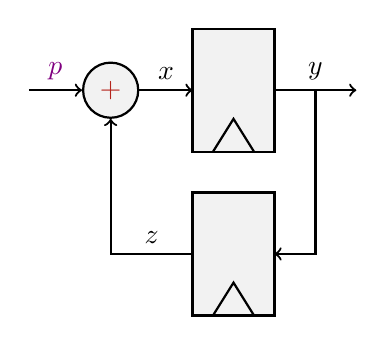
\begin{tikzpicture}[scale=0.52,thick]
    % adder
    \node[circle,draw,minimum size=.7cm,fill=gray!10] (a) at (0,0) {\textred{$+$}};
    \draw[->] (-2,0) --node[above]{\textpurple{$p$}} (a);
    \draw[->] (a) --node[above]{$x$} (2,0);
    % register1
    \draw[fill=gray!10] (2,-1.5) rectangle (4,1.5);
    \draw (2.5,-1.5) -- (3,-0.7) -- (3.5,-1.5);
    \draw[->] (4,0) --node[above]{$y$} (6,0);
    % register2
    \draw[fill=gray!10] (2,-5.5) rectangle (4,-2.5);
    \draw (2.5,-5.5) -- (3,-4.7) -- (3.5,-5.5);
    \draw[->] (5,0) -- (5,-4) -- (4,-4);
    \draw[->] (2,-4) --node[above]{$z$} (0,-4) -- (a);
\end{tikzpicture}

        \caption{The circuit under analysis.}
    \end{subfigure}
    \hfill
    \begin{subfigure}[b]{.6\textwidth}
        \centering
        \[
        \left\{ x = \textpurple{p} + z,\ y \Leftarrow x,\ z \Leftarrow y\right\}
        \]
        \caption{Formal representation of this circuit.}
        \vspace{1ex}
        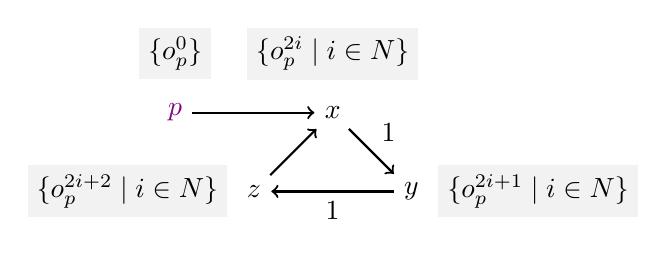
\begin{tikzpicture}[scale=1,thick]
    \node (p) at (0, 0) {$\textpurple{p}$};
    \node[fill=gray!10] at (0, 0.75) {$\{o_p^0\}$};

    \node (x) at (2, 0) {$x$};
    \node[fill=gray!10] at (2, 0.75) {$\{o_p^{2i}\mid i \in \nats\}$};

    \node (y) at (3, -1) {$y$};
    \node[fill=gray!10,right=3pt of y] {$\{o_p^{2i + 1}\mid i \in \nats\}$};

    \node (z) at (1, -1) {$z$};
    \node[fill=gray!10,left=3pt of z] {$\{o_p^{2i + 2}\mid i \in \nats\}$};

    \draw [->] (p) -- (x);
    \draw [->] (x) --node[above right]{$1$} (y);
    \draw [->] (y) --node[below]{$1$} (z);
    \draw [->] (z) -- (x);
\end{tikzpicture}

        \caption{\tia's result for this circuit.}
    \end{subfigure}
    \hfill
    \caption{An example of temporal influence analysis (\tia) with infinite temporal influence objects.}\label{fig:inf}
\end{figure}

A practical challenge in implementing \tia is that the set of temporal influence objects associated with a circuit location can be infinite.
Figure~\ref{fig:inf} illustrates such an example, where a feedback loop can propagate an input port's influence across arbitrarily many clock cycles, resulting in infinitely many temporal influence objects.
Consequently, a direct worklist algorithm that computes the fixed point of Definition~\ref{def:tia} may fail to terminate.
To address this issue, we introduce a widening operation $\widening : \powerset(\objects) \to \powerset(\objects)$ for \tia, given in Algorithm~\ref{alg:widening}.
The widening operation replaces larger sets of temporal influence objects with arithmetic progressions, which can be represented compactly using only the initial term and common difference.

Consider the successive analysis results for $\absT(y)$ in the \tia example of Figure~\ref{fig:inf}:
\[
\emptyset \xrightarrow{ \tia } \{o_p^1\} \xrightarrow{ \tia } \{o_p^1, o_p^3\} \xrightarrow{ \tia } \{o_p^1, o_p^3, o_p^5\} \xrightarrow{ \tia } \{o_p^1, o_p^3, o_p^5, o_p^7\} \xrightarrow{ \tia } \dots
\]
This sequence does not reach a finite fixed point because the set of temporal influence objects grows indefinitely.
Now consider a widening threshold of $N=3$ in
Algorithm~\ref{alg:widening}, and apply $\widening$ whenever $\absT$ changes.
After the third temporal influence object is discovered, widening replaces the finite set with the corresponding arithmetic progression:
\[
\emptyset \to \{o_p^1\} \xrightarrow{ \tia } \{o_p^1, o_p^3\} \xrightarrow{ \tia } \{o_p^1, o_p^3, o_p^5\} \xrightarrow{ \widening } \{o_p^{1+2i}\mid i \in \nats\} \xrightarrow{ \tia } \{o_p^{1+2i}\mid i \in \nats\}\ \text{(fixed point)}
\]
Thus, widening allows the analysis to represent the infinite set of temporal influence objects compactly and reach a fixed point after a finite number of iterations.

\begin{algorithm}[tp]
    \caption{Widening Operation for \tia}\label{alg:widening}
    \begin{algorithmic}[1]
        \Require a set of temporal influence objects $O$
        \Ensure a widened set of temporal influence objects $O'$ such that $O \subseteq O'$
        \State Let $N > 1$ be a threshold for triggering widening.
        \Procedure{TiaWidening}{$O$}:
        \State $O' := \emptyset$
        \ForAll{$p \in \ports$}
        \label{line:port}
        \State $O_p := \{o_p^i \in O\}$ \label{line:origin}
        \Comment{Gets the influence objects of port $p$.}
        \If{$|O_p| \ge N$} \label{line:threshold}
        \Comment{Widens $O_p$ to an arithmetic progression.}
        \State $a := \min\{i \mid o_p^i \in O_p\}$ \label{line:init}
        \Comment{Initial term.}
        \State $d := \gcd\{ |i - j | \mid o_p^i, o_p^j \in O_p\}$ \label{line:diff}
        \Comment{Common difference.}
        \State $O_p := \{o_p^{a + di} | i\in \nats\}$ \label{line:widened}
        \Comment{Represented compactly by $a$ and $d$.}
        \EndIf
        \State $O' := O' \cup O_p$
        \EndFor
        \State \Return $O'$
        \EndProcedure
    \end{algorithmic}
\end{algorithm}

\paragraph{Soundness and Convergence Property of \widening}

Next, we prove the soundness and convergence properties of this widening operation.

\begin{theorem}[Soundness of \widening]\label{theo:widening-soundness}
    The widening operation $\widening : \powerset(\objects) \to \powerset(\objects)$ defined by Algorithm~\ref{alg:widening} is sound, i.e.,
    \[
    \forall O \in \powerset(\objects).\ O \subseteq \widening(O).
    \]
\end{theorem}
\begin{proof}
    It suffices to show that, for every $p \in \ports$, the resulting set $O_p$ at Line~\ref{line:widened} is a superset of the original set $O_p$ at Line~\ref{line:origin} when widening is triggered.
    Let $O_p'$ denote the widened set at Line~\ref{line:widened}.
    Consider any $o_p^k \in O_p$.
    By Line~\ref{line:init}, $a = \min\{i \mid o_p^i \in O_p\}$, so $k-a \ge 0$.
    Moreover, by Line~\ref{line:diff}, $d = \gcd\{ |i-j| \mid o_p^i,o_p^j \in O_p\}$.
    Thus, $d$ divides $|k-a| = k-a$, and hence there exists some
    $i \in \nats$ such that $k-a = di$.
    Therefore, $k = a + di$, which implies $o_p^k \in O_p'
    = \{o_p^{a+di} \mid i \in \nats\}$.
    Hence $O_p \subseteq O_p'$.
\end{proof}

By Theorem~\ref{theo:widening-soundness}, applying $\widening : \powerset(\objects) \to \powerset(\objects)$ after each $\tia$ update of $\absT(l) \in \powerset(\objects)$ preserves soundness for every location $l$, since widening only adds temporal influence objects to $\absT(l)$ and therefore cannot remove any information established by $\tia$.

\begin{theorem}[Convergence of \widening]\label{theo:widening-convergence}
    For an arbitrary sequence of temporal influence object sets $O_0,O_1,O_2,\dots \subseteq \objects$ such that $O_0$ is finite and
    \[
    \forall i \in \nats.\ O_{i+1} = \widening(O_i \cup \{o_{p_i}^{k_i}\})
    \]
    for some $p_i \in \ports$ and $k_i \in \nats$, the sequence eventually reaches a fixed point (i.e., converges):
    \[
    \exists n \in \nats.\ O_n = O_{n+1} = O_{n+2} = \cdots.
    \]
\end{theorem}
\begin{proof}
    Without loss of generality, we first make two assumptions that simplify the proof:
    \begin{enumerate}[leftmargin=*]
        \item
        It suffices to consider the evolution of the temporal influence objects associated with a single input port $p$, since $\widening$ processes the objects associated with each input port independently by Line~\ref{line:port} of Algorithm~\ref{alg:widening}.
        Thus, we assume that every object in $O_i$ has the form $o_p^j$.
        \item
        We assume that $|O_0| \geq N$.
        If the sequence reaches a fixed point before the widening threshold is reached, the theorem already holds.
        Otherwise, since each step adds at most one new temporal influence object, the sequence reaches the threshold after finitely many steps.
        We can therefore take the first set at which widening is triggered as the new $O_0$.
    \end{enumerate}
    From this point onward, every $O_i$ ($i \ge 1$) has the form
    \[
    O_i = \{o_p^{a + d j} \mid j \in \nats\}
    \]
    for some $a,d \in \nats$.
    Now define a potential function $\varphi : \{O_i \mid i \ge 1\} \to \nats$ as
    \[
    \varphi\left(\{o_p^{a + dj} \mid j \in \nats\}\right) = a + d.
    \]
    Since $\nats$ is well ordered and therefore admits no infinite strictly decreasing sequence, it suffices to show that
    \begin{equation}\label{eq:potential}
        \forall i \ge 1.\ O_{i+1} \ne O_{i} \Rightarrow \varphi(O_{i+1}) < \varphi(O_{i}).
    \end{equation}
    This ensures that the sequence can change only finitely many times, and therefore must eventually reach a fixed point.

    \paragraph{Proof of Equation~\eqref{eq:potential}}
    Consider any $i \geq 1$ and suppose
    \[
    O_i = \{o_p^{a + d j} \mid j \in \nats\}
    \]
    and
    \[
    O_{i+1} = \widening(O_i \cup \{o_p^k\}) = \{o_p^{a'+d'j}\mid j\in\nats\}
    \]
    for some $a,d, k, a', d' \in \nats$.
    Since $O_{i+1}\neq O_i$, we must have $o_p^k\notin O_i$.
    We consider two cases:

    \noindent
    (1) Case $k < a$:
    Since $k$ is the new minimum, we have $a' = k < a$ by Line~\ref{line:init} of Algorithm~\ref{alg:widening}.
    Moreover, all differences between elements of $O_i$ are multiples of $d$, so the new common difference is $d' = \gcd(a - k, d)$ by Line~\ref{line:diff} of Algorithm~\ref{alg:widening}.
    Therefore,
    \[
    \varphi(O_{i+1}) = a' + d' < a + d' = a + \gcd(a - k, d) \le a + d = \varphi(O_i).
    \]

    \noindent
    (2) Case $k > a$:
    The new minimum remains $a$, so $a' = a$ by Line~\ref{line:init} of Algorithm~\ref{alg:widening}.
    Moreover, the new common difference $d' = \gcd(k - a, d)$ by Line~\ref{line:diff} of Algorithm~\ref{alg:widening}.
    Since $o_p^k \notin O_i$, $k-a$ is not divisible by $d$.
    Thus, $\gcd(k - a, d) < d$ and consequently
    \[
    \varphi(O_{i+1}) = a + d' = a + \gcd(a - k, d) < a + d = \varphi(O_i).
    \]
    Therefore, in both cases, $O_{i+1} \neq O_i \Rightarrow
    \varphi(O_{i+1}) < \varphi(O_i)$, which proves Equation~\eqref{eq:potential}.
\end{proof}

By Theorem~\ref{theo:widening-convergence}, applying $\widening : \powerset(\objects) \to \powerset(\objects)$ after each $\tia$ update of $\absT(l) \in \powerset(\objects)$ ensures that the evolution of $\absT(l)$ eventually reaches a fixed point for every location $l$.
Consequently, the widened version of $\tia$ eventually converges.
\subsection{Precision Discussion of \widening}

\begin{figure}[tp]
    \hfill
    \begin{subfigure}[b]{.22\textwidth}
        \centering
        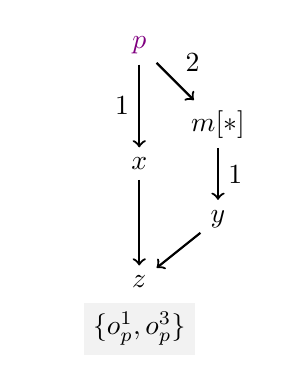
\begin{tikzpicture}[scale=1,thick]
    \node (p) at (0, 0) {$\textpurple{p}$};
    \node (x) at (0, -1.5) {$x$};
    \node (m) at (1, -1) {$m[*]$};
    \node (y) at (1, -2.2) {$y$};
    \node (z) at (0, -3) {$z$};

    \draw [->] (p) --node[left]{$1$} (x);
    \draw [->] (x) -- (z);
    \draw [->] (p) --node[above right]{$2$} (m);
    \draw [->] (m) --node[right]{$1$} (y);
    \draw [->] (y) -- (z);

    \node at (-1.3, 0) {};

    \node[fill=gray!10] (t) at (0, -3.6) {$\{o_p^1, o_p^3\}$};
\end{tikzpicture}

        \caption{Acyclic Pattern.}\label{fig:acyclic-pattern}
    \end{subfigure}
    \hfill
    \begin{subfigure}[b]{.31\textwidth}
        \centering
        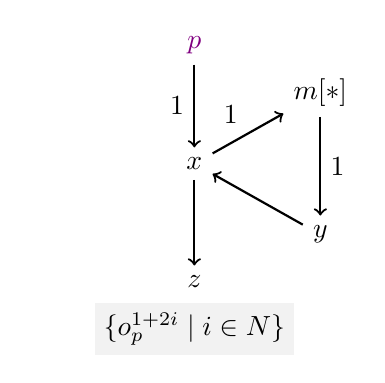
\begin{tikzpicture}[scale=1,thick]
    \node (p) at (0, 0) {$\textpurple{p}$};
    \node (x) at (0, -1.5) {$x$};
    \node (m) at (1.6, -0.6) {$m[*]$};
    \node (y) at (1.6, -2.4) {$y$};
    \node (z) at (0, -3) {$z$};
    \node[fill=gray!10] at (0, -3.6) {$\{o_p^{1 + 2i} \mid  i \in \nats\}$};

    \draw [->] (p) --node[left]{$1$} (x);
    \draw [->] (x) --node[above left]{$1$} (m);
    \draw [->] (m) --node[right]{$1$} (y);
    \draw [->] (y) -- (x);
    \draw [->] (x) -- (z);

    \node at (-2, 0) {};
\end{tikzpicture}

        \caption{Single-Cycle Pattern.}\label{fig:single-cycle-pattern}
    \end{subfigure}
    \hfill
    \hfill
    \begin{subfigure}[b]{.32\textwidth}
        \centering
        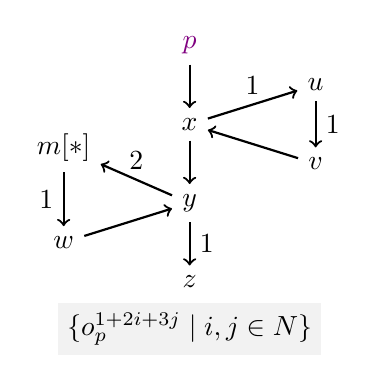
\begin{tikzpicture}[scale=1,thick]
    \node (p) at (0, 0) {$\textpurple{p}$};
    \node (x) at (0, -1) {$x$};
    \node (u) at (1.6, -0.5) {$u$};
    \node (v) at (1.6, -1.5) {$v$};
    \node (y) at (0, -2) {$y$};
    \node (m) at (-1.6, -1.3) {$m[*]$};
    \node (w) at (-1.6, -2.5) {$w$};



    \node (z) at (0, -3) {$z$};
    \node[fill=gray!10] at (0, -3.6) {$\{o_p^{1 + 2i + 3j} \mid  i, j \in \nats\}$};

    \draw [->] (p) -- (x);
    \draw [->] (x) --node[above]{$1$} (u);
    \draw [->] (u) --node[right]{$1$} (v);
    \draw [->] (v) -- (x);
    \draw [->] (x) -- (y);
    \draw [->] (y) --node[above]{$2$} (m);
    \draw [->] (m) --node[left]{$1$} (w);
    \draw [->] (w) -- (y);
    \draw [->] (y) --node[right]{$1$} (z);
\end{tikzpicture}

        \caption{Multiple-Cycle Pattern.}\label{fig:multiple-cycles-pattern}
    \end{subfigure}
    \hfill
    \caption{
        Representative TIG patterns for discussing the precision of \widening, focusing on $\absT(z)$ for simplicity.
        The ideal \tia results without \widening are shown in gray boxes.
    }\label{fig:precision-pattern}.
\end{figure}

In this section, we discuss the precision trade-off introduced by $\widening$ to ensure convergence.
For simplicity, we focus on the temporal influence objects associated with a single input port $p$, since $\widening$ processes each port independently (Line~\ref{line:port} of Algorithm~\ref{alg:widening}).
Figure~\ref{fig:precision-pattern} illustrates three representative TIG patterns and their corresponding ideal \tia results without \widening.
We next examine how applying $\widening$ affects the precision of \tia for each pattern.

\paragraph{Acyclic Pattern}

As illustrated in Figure~\ref{fig:acyclic-pattern}, when all paths in the TIG from input port $p$ to location $z$ are acyclic, $\absT(z)$ is finite.
Therefore, if the widening threshold is sufficiently large such that $N > |\absT(z)|$, $\widening$ is never triggered for $\absT(z)$, and $\widening(\absT(z)) = \absT(z)$ by Line~\ref{line:threshold} of Algorithm~\ref{alg:widening}.
Thus, widening introduces no precision loss in this case.
Theoretically, such an $N$ always exists because $\absT(z)$ is finite.
However, determining the smallest such threshold in general would require computing the precise temporal influence information, which is precisely the information that the analysis is intended to approximate.
In practice, we therefore choose a sufficiently large fixed threshold rather than computing a circuit-specific threshold.

Moreover, the number of distinct propagation delays along acyclic TIG paths between two circuit locations is typically expected to remain relatively small in synchronous hardware designs.
For example, the two incoming TIG edges to $z$ in Figure~\ref{fig:acyclic-pattern} can only arise from a wire connection such as $z = x \mathbin{\vop} y$ (where $\vop$ is an operator) through rule~\rTiaWire.
In typical designs, the operands of such expressions combine a limited number of paths with different pipeline depths, rather than intentionally combining a large number of distinct propagation delays.
Thus, when $\absT(z)$ is finite, its cardinality is generally expected to remain manageable for a reasonably large widening threshold.

\paragraph{Single Cycles Pattern}

As illustrated in Figure~\ref{fig:single-cycle-pattern}, suppose that all paths from $p$ to $z$ contain at most one cycle, and that the cycle has propagation delay $d$.
Traversing the cycle an arbitrary number of times produces temporal influence objects whose delays form an arithmetic progression.
In particular, for some minimum delay $a$, $\absT(z) = \{o_p^{a + di} \mid i \in \nats\}$.
Consequently, when widening is triggered, Lines~\ref{line:init}--\ref{line:widened} of Algorithm~\ref{alg:widening} recover exactly the same arithmetic progression.
For the example in Figure~\ref{fig:single-cycle-pattern},
\[
\begin{aligned}
    \widening(\absT(z)) & = \widening(\{o_p^{1+2i} \mid i\in \nats\})\\
    & = \widening(\{o_p^1, o_p^3, o_p^5, \dots\}) = \{o_p^{1+2i} \mid i \in \nats\} = \absT(z).\\
\end{aligned}
\]
So, widening introduces no precision loss for this pattern either.

\paragraph{Multiple Cycles Pattern}

The precision behavior becomes more interesting when multiple cycles with different propagation delays occur along TIG paths from $p$ to $z$, as illustrated in Figure~\ref{fig:multiple-cycles-pattern}.
In this case, temporal influences can traverse each cycle an arbitrary number of times, and the resulting temporal influence set is generally not itself an arithmetic progression.
For the example in Figure~\ref{fig:multiple-cycles-pattern}, the path contains cycles with propagation delays $2$ and $3$, and the acyclic portion of the path contributes a minimum delay of $1$.
By rule $\rTiaPropa$, the resulting temporal influence set is
\[
\absT(z)=\{o_p^{1+2i+3j}\mid i,j\in\nats\}.
\]
Thus by Line~\ref{line:init}--\ref{line:widened} of Algorithm~\ref{alg:widening} we have:
\[
\begin{aligned}
    \widening(\absT(z)) & = \widening(\{o_p^{1+2i+3j} \mid i, j\in \nats\})\\
    & = \widening(\{o_p^1, o_p^3, o_p^4, o_p^5, o_p^6 \dots\}) = \{o_p^{1+i} \mid i \in \nats\}.\\
\end{aligned}
\]
Hence, in this example, widening introduces only one false positive, namely $o_p^2$:
\[
\widening(\absT(z))-\absT(z)=\{o_p^2\}.
\]
This observation generalizes to arbitrary multiple-cycle patterns.
In such patterns, the temporal influence propagation delays generated by a finite collection of cycles can be expressed as additive combinations of their cycle delays, offset by the minimum delay along a path that traverses none of the cycles.
The following lemma shows that, although $\widening$ may introduce false positives for such infinite sets, it introduces only finitely many of them.

\begin{lemma}[Finite Precision Loss of \widening for Multiple-Cycle Patterns]\label{lem:finite-widening}
    Given a minimum propagation delay $a_0 \in \nats$ and repeatable cycle delays $0 < a_1 < a_2 < \dots < a_n \in \nats$ with $n > 1$, for $p \in \ports$, let
    \[
    O_p = \left\{ o_p^k \mid  \exists i_1,\dots,i_n \in \nats.\ k = a_0 + \sum_{r=1}^{n} a_r i_r \right\}.
    \]
    Then $\widening(O_p) - O_p$ is finite.
\end{lemma}
\begin{proof}
    Let $g = \gcd(a_1,\dots,a_n)$.
    Since $a_0 \in O_p$ and $a_0+a_r \in O_p$ for every $1 \le r \le n$, the common difference computed by $\widening$ (Line~\ref{line:diff} of Algorithm~\ref{alg:widening}) is exactly $g$.
    Moreover, $a_0$ is the minimum element of $O_p$.
    Therefore,
    \[
    \widening(O_p) = \{ o_p^{a_0+gi} \mid i\in\nats \}.
    \]
    Let $b_r=a_r/g$ for $1\le r\le n$.
    Then $\gcd(b_1,\dots,b_n)=1$.
    Consider the additive monoid generated by $b_1,\dots,b_n$:
    \[
    M = \left\{ \sum_{r=1}^{n} b_r i_r \mid i_1,\dots,i_n\in\nats \right\}.
    \]
    Since the generators have greatest common divisor $1$, $M$ is a numerical semigroup and is cofinite in $\nats$~\cite{rosales_numerical_2009};
    that is, there exists some $B\in\nats$ such that every $i\ge B$ belongs to $M$.
    Thus,
    \[
    \forall i \ge B.\ \exists i_1,\dots,i_n\in\nats.\ a_0+gi = a_0+g\sum_{r=1}^{n}b_r i_r = a_0+g\sum_{r=1}^{n}\frac{a_r}{g}\cdot i_r = a_0+\sum_{r=1}^{n}a_r i_r,
    \]
    which implies
    \[
    \forall i \ge B.\ o_p^{a_0+gi}\in O_p.
    \]
    Therefore, all but finitely many elements of $\widening(O_p)$ already belong to $O_p$.
    In particular,
    \[
    \widening(O_p) - O_p \subseteq \{ o_p^{a_0+gi} \mid 0\le i<B \},
    \]
    which is finite.
\end{proof}

\paragraph{Summary}
The three patterns discussed above illustrate the precision behavior of $\widening$.
For acyclic patterns, $\widening$ introduces no precision loss provided that the widening threshold exceeds the finite number of distinct temporal influence objects.
For single-cycle patterns, the temporal influence set is already an arithmetic progression, so $\widening$ is exact and preserves precision.
For multiple-cycle patterns, $\widening$ may introduce false positives, but Lemma~\ref{lem:finite-widening} shows that only finitely many false positives can be introduced.



\section{Practical Potential of \tia}\label{sec:clients}

To demonstrate \tia's practical potential to support diverse hardware analysis clients, we develop three client analyses on top of it: detecting signal asynchrony bugs (Section~\ref{sec:client-asynchrony}) for hardware bug detection, identifying timing-flow information leaks (Section~\ref{sec:client-timingflow}) for hardware security analysis, and inferring timeline intervals (Section~\ref{sec:client-timeline}) for hardware design understanding.

\subsection{Detecting Signal Asynchrony Bugs}\label{sec:client-asynchrony}

\begin{figure}[tp]
    \hfill
    \begin{subfigure}[b]{.45\textwidth}
        \begin{subfigure}{\linewidth}
            \centering
            \begin{chisel}
val request           = Input(Bool())
val data              = Input(UInt(32.W))
val response          = Reg(UInt(32.W))
val valid             = Reg(Bool())
// --- Simplifed Design Logic ---
val buffered_response = Reg(UInt(32.W))
+ val buffered_valid  = Reg(Bool())
when (request) {
    buffered_response := data
}
response := buffered_response
- when (request) {
    -     valid := true.B
    - }
+ when (request) {
    +     buffered_valid := true.B
    + }
+ valid := buffered_valid
            \end{chisel}
            \caption{A bug-fixing commit for signal asynchrony.}
            \label{fig:asynchrony-code}
        \end{subfigure}

        \vspace{1ex}

        \begin{subfigure}{\linewidth}
            \centering
            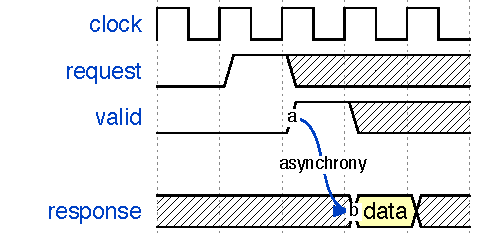
\includegraphics[width=\linewidth,clip,trim=20 0 10 0]{figures/asynchrony-waveform}
            \caption{Waveform illustrating the asynchrony between \texttt{valid} and \texttt{response} after a request.}
            \label{fig:asynchrony-waveform}
        \end{subfigure}
    \end{subfigure}
    \hfill
    \begin{subfigure}[b]{.53\textwidth}
        \begin{subfigure}{\linewidth}
            \centering
            \footnotesize
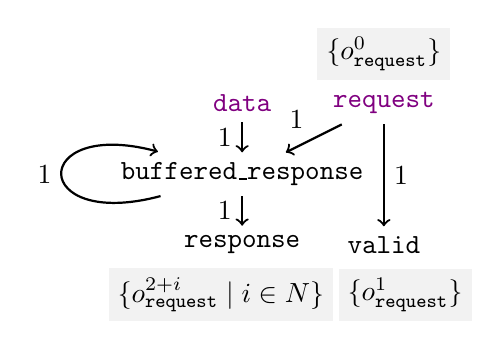
\begin{tikzpicture}[scale=.9,thick]
    \node (d) at (0, 0) {$\textpurple{\mathtt{data}}$};
    \node (rq) at (2, 0) {$\textpurple{\mathtt{request}}$};

    \node (br) at (0, -1) {$\mathtt{buffered\_response}$};
    \node (rp) at (0, -2) {$\mathtt{response}$};
    \node (v)  at (2, -2) {$\mathtt{valid}$};

    \draw[->] (d) -- node[left]{$1$} (br);
    \draw[->] (rq) -- node[above left]{$1$} (br);
    \draw[->] (br) edge[loop left] node{$1$} (br);
    \draw[->] (br) -- node[left]{$1$} (rp);
    \draw[->] (rq) -- node[right]{$1$} (v);


    \node[fill=gray!10] at (2, .7) {$\{o_{\mathtt{request}}^0\}$};
    \node[fill=gray!10] at (-.3, -2.7) {$\{o_{\mathtt{request}}^{2+i}\mid i\in\nats\}$};
    \node[fill=gray!10] at (2.3, -2.7) {$\{o_{\mathtt{request}}^1\}$};
\end{tikzpicture}

            \caption{\tia results before the bug fix, showing \emph{asynchronous} temporal influences of \texttt{request} on \texttt{response} and \texttt{valid}.}\label{fig:tia-asynchrony}
        \end{subfigure}

        \vspace{1ex}

        \begin{subfigure}{\linewidth}
            \centering
            \footnotesize
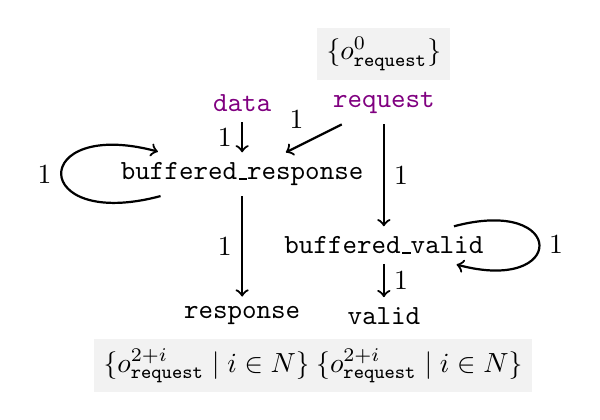
\begin{tikzpicture}[scale=.9,thick]
    \node (d) at (0, 0) {$\textpurple{\mathtt{data}}$};
    \node (rq) at (2, 0) {$\textpurple{\mathtt{request}}$};

    \node (br) at (0, -1) {$\mathtt{buffered\_response}$};
    \node (rp) at (0, -3) {$\mathtt{response}$};
    \node (bv)  at (2, -2) {$\mathtt{buffered\_valid}$};
    \node (v)  at (2, -3) {$\mathtt{valid}$};

    \draw[->] (d) -- node[left]{$1$} (br);
    \draw[->] (rq) -- node[above left]{$1$} (br);
    \draw[->] (br) edge[loop left] node{$1$} (br);
    \draw[->] (br) -- node[left]{$1$} (rp);
    \draw[->] (rq) -- node[right]{$1$} (bv);
    \draw[->] (bv) -- node[right]{$1$} (v);
    \draw[->] (bv) edge[loop right] node{$1$} (bv);


    \node[fill=gray!10] at (2, .7) {$\{o_{\mathtt{request}}^0\}$};
    \node[fill=gray!10] at (-.5, -3.7) {$\{o_{\mathtt{request}}^{2+i}\mid i\in\nats\}$};
    \node[fill=gray!10] at (2.5, -3.7) {$\{o_{\mathtt{request}}^{2+i}\mid i \in \nats\}$};
\end{tikzpicture}

            \caption{\tia results after the bug fix, showing \emph{synchronous} temporal influences of \texttt{request} on \texttt{response} and \texttt{valid}.}\label{fig:tia-synchrony}
        \end{subfigure}

        \vspace{1ex}

        \begin{subfigure}{\linewidth}
            \centering
            \footnotesize
            \[
            \begin{aligned}
                & \min\left\{i \mid o_{\mathtt{request}}^{i} \in \absT(\mathtt{response})\right\} \\
                \ne &\min\left\{i \mid o_{\mathtt{request}}^{i} \in \absT(\mathtt{valid})\right\} \\
            \end{aligned}
            \]
            \caption{An observation guiding signal asynchrony analysis.}
            \label{fig:asynchrony-observe}
        \end{subfigure}
    \end{subfigure}
    \hfill
    \caption{A motivating example for signal asynchrony analysis.}
\end{figure}

A \emph{signal asynchrony} bug occurs when two variables that are intended to be used together---such as a data variable and its associated valid or backpressure signal, or the two operands of a mathematical operation---are not updated synchronously~\cite{ma_debugging_2022}.
We'll first introduce signal asynchrony bugs through a simplified example and then describe how our signal asynchrony analysis detect such bugs leveraging the fundamental temporal influence information provided by \tia.

\paragraph{Example of A Signal Asynchrony Bug}

Figure~\ref{fig:asynchrony-code} shows a simplified Chisel example adapted from a bug-fixing commit~\cite{aysnchrony-fix-commit} for a signal asynchrony bug.
Deleted code is shown in red, while newly added code is shown in green.
The code describes a hardware design that responds to requests that requires a minimum two-cycle latency between each request (Line~1) and its corresponding response (Lines~3--4).
Upon receiving a request, the code therefore buffers the response, which can be computed in a single cycle, for one additional cycle in \texttt{buffered\_response} (Lines~8--10) before assigning it to the output \texttt{response} (Line~11).
However, in the buggy version, the \texttt{valid} signal, which indicates that \texttt{response} is valid, is asserted immediately upon receiving the request (Lines~12--14).
Consequently, \texttt{valid} becomes asserted one cycle before the corresponding \texttt{response} becomes valid, resulting in a signal asynchrony bug.
For simplicity, we omit the code that resets \texttt{valid} to 0.
Figure~\ref{fig:asynchrony-waveform} illustrates this asynchrony between \text{valid} and \text{response} after a request in the waveform.
The bug can be fixed by delaying \texttt{valid} by one cycle so that it becomes synchronized with \texttt{response}.
As shown in Figure~\ref{fig:asynchrony-code}, the developer introduces an intermediate register \texttt{buffered\_valid} (Line~7), assigns \texttt{valid} from it (Line~18), and replaces the original assignments to \texttt{valid} (Lines~12--14) with assignments to \texttt{buffered\_valid} (Lines~15--17).

\paragraph{Insights of Signal Asynchrony Analysis}

Figure~\ref{fig:tia-asynchrony} and Figure~\ref{fig:tia-synchrony} show the \tia results for the circuit in Figure~\ref{fig:asynchrony-code} before and after the signal asynchrony bug fix, respectively, focusing on how \texttt{request} temporally influences \texttt{response} and \texttt{valid}.
Before the fix, as shown in Figure~\ref{fig:tia-asynchrony}, the minimum temporal influence that \texttt{response} receives from \texttt{request} is two cycles, whereas that of \texttt{valid} is one cycle, indicating that the two signals are asynchronous with respect to \texttt{request}.
After the fix, as shown in Figure~\ref{fig:tia-synchrony}, both signals receive the same minimum temporal influence from \texttt{request}.
This observation is formally summarized in Figure~\ref{fig:asynchrony-observe}.

Guided by this observation, we generalize the \texttt{request} signal to an arbitrary synchronizer signal $p \in \ports$ and \texttt{response} and \texttt{valid} to arbitrary synchronized signals $x,y \in \variables$.
Our \emph{signal asynchrony analysis} reports that $x$ and $y$ are asynchronous with respect to $p$ if
\begin{equation}\label{eq:asynchrony}
    \min\left\{i \mid o_p^i \in \absT(x)\right\}
    \ne
    \min\left\{i \mid o_p^i \in \absT(y)\right\},
\end{equation}
where $\absT$ is the temporal influence information computed by \tia.

For practility, we compare the minimum temporal influences rather than the entire temporal influence sets in Equation~\ref{eq:asynchrony}.
In principle, comparing the entire sets would report asynchrony whenever the two signals have any difference in their temporal influence sets.
However, we observe in practice that this criterion is overly restrictive and kills many fine designs (i.e., falgs many false positive bugs), because two signals may have different temporal influence sets while still being sufficiently synchronized for their intended use.
The minimum temporal influence provides a simple and representative measure of when a signal can first become responsive to the synchronizer signal.
We therefore deliberately adopt this weaker criterion to reduce analysis noise and make the resulting reports more practical for hardware developers.


\subsection{Identifying Timing-flow Information Leaks}\label{sec:client-timingflow}

\begin{figure}[tp]
    \hfill
    \begin{subfigure}[b]{.5\textwidth}
        \begin{subfigure}{\linewidth}
            \centering
            \begin{chisel}
val dividend     = Input(UInt(32.W))
val divisor      = Input(UInt(32.W))
val quotient     = Reg(UInt(32.W))
val valid        = Reg(Bool())
// --- Simplified Design Logic ---
val reg_dividend = Reg(UInt(32.W))
val reg_divisor  = Reg(UInt(32.W))
when (reg_dividend >= reg_divisor) {
    reg_dividend := reg_dividend - reg_divisor
    quotient     := quotient + 1.U
} otherwise {
    valid        := true.B
}
            \end{chisel}
            \caption{A simplified Chisel example exhibiting a timing flow from the secret \texttt{divisor} to the observable \texttt{valid}.}
            \label{fig:timingflow-code}
        \end{subfigure}

        \vspace{1ex}

        \begin{subfigure}{\linewidth}
            \centering
            \footnotesize
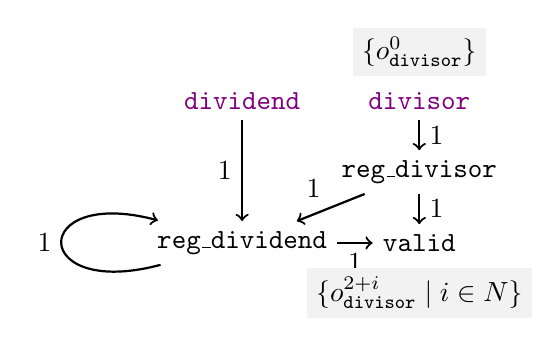
\begin{tikzpicture}[scale=.9,thick]
    \node (dd) at (0, 0) {$\textpurple{\mathtt{dividend}}$};
    \node (dr) at (2.5, 0) {$\textpurple{\mathtt{divisor}}$};

    \node (rdd) at (0, -2) {$\mathtt{reg\_dividend}$};
    \node (rdr) at (2.5, -1) {$\mathtt{reg\_divisor}$};
    \node (v)  at (2.5, -2) {$\mathtt{valid}$};

    \draw[->] (dd) -- node[left]{$1$} (rdd);
    \draw[->] (rdd) edge[loop left] node{$1$} (rdd);
    \draw[->] (rdr) -- node[above left]{$1$} (rdd);
    \draw[->] (rdd) -- node[below]{$1$} (v);

    \draw[->] (dr) -- node[right]{$1$} (rdr);
    \draw[->] (rdr) -- node[right]{$1$} (v);

    \node[fill=gray!10] at (2.5, .7) {$\{o_{\mathtt{divisor}}^0\}$};
    \node[fill=gray!10] at (2.5, -2.7) {$\{o_{\mathtt{divisor}}^{2+i}\mid i\in\nats\}$};
\end{tikzpicture}

            \caption{\tia results showing various temporal influences from the secret \texttt{divisor} to the observable \texttt{valid}.}
            \label{fig:tia-timingflow}
        \end{subfigure}


    \end{subfigure}
    \hfill
    \begin{subfigure}[b]{.46\textwidth}
        \begin{subfigure}{\linewidth}
            \centering
            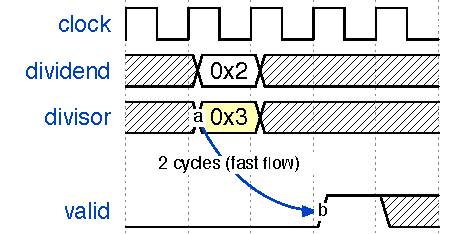
\includegraphics[width=\linewidth,clip,trim=10 0 10 0]{figures/timingflow-fast-waveform}
            \caption{Waveform illustrating a \emph{fast} flow from \texttt{divisor} to \texttt{valid}.}
            \label{fig:timingflow-waveform-fast}
        \end{subfigure}

        \vspace{1ex}

        \begin{subfigure}{\linewidth}
            \centering
            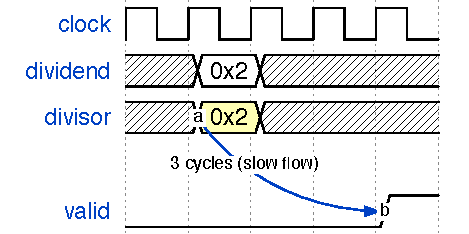
\includegraphics[width=\linewidth,clip,trim=10 0 10 0]{figures/timingflow-slow-waveform}
            \caption{Waveform illustrating a \emph{slow} flow from \texttt{divisor} to \texttt{valid}.}
            \label{fig:timingflow-waveform-slow}
        \end{subfigure}

        \vspace{1ex}

        \begin{subfigure}{\linewidth}
            \centering
            \[
            \left|\left\{o_{\mathtt{divisor}}^i \in \absT(\mathtt{valid})\right\}\right| > 1
            \]
            \caption{An observation guiding timing flow analysis.}
            \label{fig:timingflow-observe}
        \end{subfigure}
    \end{subfigure}
    \hfill
    \caption{A motivating example for timing-flow analysis.}
\end{figure}

A \emph{timing flow} is a form of implicit information flow in which sensitive information affects the timing of public hardware behavior, potentially enabling information leakage~\cite{hu_hardware_2022,ardeshiricham_clepsydra_2017,qin_formal_2020}.
We first illustrate timing flows through a simplified example and then describe how our timing-flow analysis detects them leveraging the fundamental temporal influence information provided by \tia.

\paragraph{Example of A Timing Flow}

Figure~\ref{fig:timingflow-code} shows a simplified Chisel example exhibiting the timing flow described by~\cite{ardeshiricham_clepsydra_2017}.
The circuit computes \texttt{quotient} (Line~3) from the given \texttt{dividend} (Line~1) and \texttt{divisor} (Line~2) using consecutive subtraction (Lines~6--13), with \texttt{valid} (Line~4) indicating when the computation has completed.
For simplicity, we omit the initialization logic that takes one cycle to load \texttt{dividend} into \texttt{reg\_dividend}, \texttt{divisor} into \texttt{reg\_divisor}, and reset \texttt{valid} to \texttt{false}.
Figures~\ref{fig:timingflow-waveform-fast} and~\ref{fig:timingflow-waveform-slow} illustrate how different values of \texttt{divisor} can cause \texttt{valid} to be asserted at different times, thereby creating a timing flow from \texttt{divisor}\footnote{A similar timing flow exists from \texttt{dividend} to \texttt{valid}; we focus on \texttt{divisor} for simplicity.} to \texttt{valid}.
For a fixed \texttt{dividend = 2}, consider two possible values of \texttt{divisor}.
When \texttt{divisor = 3}, the computation completes after two cycles: the first cycle initializes the registers, and the second cycle evaluates Line~8 as false and asserts \texttt{valid} at Line~12.
This corresponds to the \emph{fast} flow shown in Figure~\ref{fig:timingflow-waveform-fast}.
In contrast, when \texttt{divisor = 2}, Line~8 evaluates to true in the second cycle, causing one subtraction at Lines~9--10.
The computation therefore requires an additional cycle before \texttt{valid} is asserted by Line~12, resulting in the \emph{slow} flow shown in Figure~\ref{fig:timingflow-waveform-slow}.

Next we'll describe how such a timing flow from \texttt{divisor} to \texttt{dividend} can lead to information leak.
Consider a security scenario in which the design is open source, \texttt{dividend} is public, and \texttt{divisor} is a secret key.
Suppose an attacker cannot observe the computed \texttt{quotient}, but can measure the number of clock cycles between providing the inputs and observing \texttt{valid}.
For the slow-flow case, the attacker observes three cycles: one initialization cycle, one subtraction cycle, and one cycle in which \texttt{valid} is asserted.
Because the algorithm is known, the attacker can therefore infer that
\[
\mathtt{divisor} \leq \mathtt{dividend}
< 2\cdot\mathtt{divisor},
\]
which, for $\mathtt{dividend}=2$, implies $\mathtt{divisor}=2$.
For the fast-flow case, the attacker can at least infer that $\mathtt{divisor} > \mathtt{dividend}$.
Thus, the timing of \texttt{valid} reveals information about the secret \texttt{divisor}.
If \texttt{valid} were asserted after the same number of cycles for every possible \texttt{divisor}, no such timing-based leakage would occur.

\paragraph{Insights of Timing-flow Analysis}

Figure~\ref{fig:tia-timingflow} shows the \tia results for the circuit in Figure~\ref{fig:timingflow-code}, focusing on how \texttt{divisor} temporally influences \texttt{valid}.
We can observe that \texttt{divisor} can influence \texttt{valid} after multiple distinct numbers of clock cycles.
These distinct temporal influences correspond to the different timing behaviors illustrated in Figures~\ref{fig:timingflow-waveform-fast} and~\ref{fig:timingflow-waveform-slow}, providing an indication of the timing flow from \texttt{divisor} to \texttt{valid}.
This observation is summarized in Figure~\ref{fig:timingflow-observe}.

Guided by this observation, we generalize \texttt{divisor} to an arbitrary secret source signal $p\in\ports$ and \texttt{valid} to an arbitrary observable sink signal $x\in\variables$.
Our \emph{timing-flow analysis} reports a timing flow from $p$ to $x$ if
\[
\left|\left\{o_p^i \in \absT(x)\right\}\right| > 1,
\]
where $\absT$ is the temporal influence information computed by \tia.
Intuitively, this criterion identifies whether the same source can affect the sink after more than one number of clock cycles, indicating that the source may influence the timing of the sink.

\subsection{Understanding Timeline Interfaces}\label{sec:client-timeline}

A \emph{timeline interface} assigns each input or output of a hardware module a \emph{timeline type}~\cite{nigam_modular_2023} that specifies the clock-cycle intervals during which the corresponding signal is required or available.
Such information is important for hardware developers to \emph{understand} how to correctly use a module.
However, Chisel does not provide a type system with timeline types that explicitly encode this temporal information.
Consequently, developers must typically obtain it from documentation, build scripts, or, in the worst case, the module's implementation.
As a final client analysis built on top of \tia, we develop \emph{timeline interface analysis}, which automatically computes an approximation of a module's actual timeline interface.
Although our analysis cannot automatically and precisely equip existing Chisel codebases with the informative timeline type system, we believe that even an approximate timeline interface can still be help helpful for developers to \emph{understand} the temporal behavior of a module by making it more explicit.
We first illustrate the notion of a timeline interface through a simplified example and then describe how our timeline interface analysis approximates such interfaces from the temporal influence information computed by \tia.

\begin{figure}[tp]
    \hfill
    \begin{subfigure}[b]{.45\textwidth}
        \begin{subfigure}{\linewidth}
            \centering
            \begin{chisel}
class AU extends Module {
    val a         = Input(UInt(32.W))
    val b         = Input(UInt(32.W))
    val a_plus_b  = Output(UInt(32.W))
    val a_plus_2b = Output(UInt(32.W))
    // --- Compute a + b ---
    val reg_a  = Reg(UInt(32.W))
    val reg_b  = Reg(UInt(32.W))
    reg_a     := a
    reg_b     := b
    a_plus_b  := reg_a + reg_b
    // --- Compute a + 2b ---
    val reg_a_plus_b = Reg(UInt(32.W))
    val reg_reg_b    = Reg(UInt(32.W))
    reg_a_plus_b := a_plus_b
    reg_reg_b    := reg_b
    a_plus_2b := reg_a_plus_b + reg_reg_b
}
            \end{chisel}
            \caption{A simple Chisel arithmetic unit \texttt{AU}.}
            \label{fig:timeline-code}
        \end{subfigure}

        \vspace{1ex}

        \begin{subfigure}{\linewidth}
            \centering
            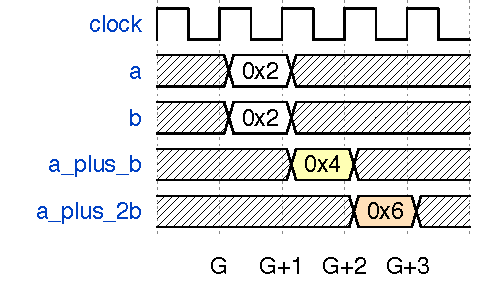
\includegraphics[width=\linewidth,clip,trim=15 15 12 0]{figures/timeline-waveform}
            \caption{Waveform illustrating the temporal behavior of \texttt{AU}, where $G$ denotes any clock-cycle time.}
            \label{fig:timeline-waveform}
        \end{subfigure}


    \end{subfigure}
    \hfill
    \begin{subfigure}[b]{.5\textwidth}
        \begin{subfigure}{\linewidth}
            \centering
            \[
            \begin{aligned}
                \forall G.\ & \textpurple{\mathtt{a}} \in [G, G+1) \wedge \textpurple{\mathtt{b}} \in [G, G+1) \\
                \Rightarrow\ & \textblue{\mathtt{a\_plus\_b}} \in [G+1, G+2)\\
                & \wedge \textblue{\mathtt{a\_plus\_2b}} \in [G+2, G+3)
            \end{aligned}
            \]
            \caption{The timeline interface of \texttt{AU}, expressed as a proposition about its temporal behavior, where $x \in [G+i,G+j)$ means that $x$ is valid from clock cycle $G+i$ through, but not including, clock cycle $G+j$.}
            \label{fig:timeline-interface}
        \end{subfigure}

        \vspace{1ex}

        \begin{subfigure}{\linewidth}
            \centering
            \footnotesize
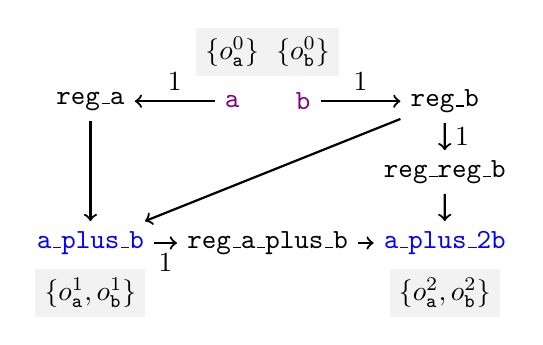
\begin{tikzpicture}[scale=.9,thick]
    \node (a) at (2, 0) {$\textpurple{\mathtt{a}}$};
    \node (b) at (3, 0) {$\textpurple{\mathtt{b}}$};
    \node (ra) at (0, 0) {$\mathtt{reg\_a}$};
    \node (rb) at (5, 0) {$\mathtt{reg\_b}$};
    \node (rrb) at (5, -1) {$\mathtt{reg\_reg\_b}$};
    \node (ab) at (0, -2) {$\textblue{\mathtt{a\_plus\_b}}$};
    \node (rab) at (2.5, -2) {$\mathtt{reg\_a\_plus\_b}$};
    \node (a2b) at (5, -2) {$\textblue{\mathtt{a\_plus\_2b}}$};

    \draw [->] (a) --node[above]{$1$} (ra);
    \draw [->] (ra) -- (ab);
    \draw [->] (rb) -- (ab);
    \draw [->] (b) --node[above]{$1$} (rb);
    \draw [->] (rb) --node[right]{$1$} (rrb);
    \draw [->] (ab) --node[below]{$1$} (rab);
    \draw [->] (rab) -- (a2b);
    \draw [->] (rrb) -- (a2b);

    \node[fill=gray!10] at (2, .7) {$\{o_{\mathtt{a}}^0\}$};
    \node[fill=gray!10] at (3, .7) {$\{o_{\mathtt{b}}^0\}$};

    \node[fill=gray!10] at (0, -2.7) {$\{o_{\mathtt{a}}^1, o_{\mathtt{b}}^1\}$};
    \node[fill=gray!10] at (5, -2.7) {$\{o_{\mathtt{a}}^2, o_{\mathtt{b}}^2\}$};
\end{tikzpicture}

            \caption{\tia results showing the temporal influences of \texttt{AU}'s inputs (purple) on its outputs (blue).}
            \label{fig:tia-timeline}
        \end{subfigure}

        \vspace{1ex}

        \begin{subfigure}{\linewidth}
            For all $G$, let $I_G(x)$ be the \emph{minimal} interval $[G+i, G+j)$ that \emph{contains}
            \[
            \left\{G + i \mid \exists p \in \ports.\ o_p^i \in \absT(x)\right\}.
            \]
            We observe
            \[
            \textblue{\mathtt{a\_plus\_b}} \in [G + 1, G + 2) \subseteq I_G(\textblue{\mathtt{a\_plus\_b}})
            \]
            and
            \[
            \textblue{\mathtt{a\_plus\_2b}} \in [G + 2, G + 3) \subseteq I_G(\textblue{\mathtt{a\_plus\_2b}}).
            \]
            \caption{An observation guiding timeline interface analysis.}
            \label{fig:timeline-observe}
        \end{subfigure}
    \end{subfigure}
    \hfill
    \caption{A motivating example for timeline interface analysis.}
\end{figure}

\paragraph{Example of a Timeline Interface}

Figure~\ref{fig:timeline-code} shows a simple Chisel arithmetic unit \texttt{AU} (Line~1) with inputs \texttt{a} and \texttt{b} (Lines~2--3) and outputs \texttt{a\_plus\_b} and \texttt{a\_plus\_2b} (Lines~4--5).
The module takes one clock cycle to compute $\mathtt{a}+\mathtt{b}$ and produces the result at \texttt{a\_plus\_b} (Lines~6--11).
It then takes another cycle to compute $\mathtt{a}+2\mathtt{b}$ and produces the result at \texttt{a\_plus\_2b} (Lines~12--17).
Figure~\ref{fig:timeline-waveform} visualizes this temporal behavior, where $G$ denotes a generic clock-cycle time at which the inputs are provided to \texttt{AU}.

Figure~\ref{fig:timeline-interface} summarizes this behavior as a timeline interface.
Specifically, if the user provides \texttt{a} and \texttt{b} during $[G,G+1)$, then \texttt{a\_plus\_b} becomes available during $[G+1,G+2)$, while \texttt{a\_plus\_2b} becomes available during $[G+2,G+3)$.
With this timeline interface, a user can \emph{understand} when the outputs of \texttt{AU} become available without inspecting its implementation.

\paragraph{Insights of Timeline Interface Analysis}

Figure~\ref{fig:tia-timeline} shows the \tia results for the \texttt{AU} module in Figure~\ref{fig:timeline-code}, focusing on its inputs and outputs.
We observe that \texttt{a\_plus\_b} can be influenced by an input only after one cycle, whereas \texttt{a\_plus\_2b} can be influenced by an input only after two cycles.
Assuming that both \texttt{a} and \texttt{b} are provided during $[G,G+1)$, this temporal influence information implies that \texttt{a\_plus\_b} becomes available during $[G+1,G+2)$ and \texttt{a\_plus\_2b} during $[G+2,G+3)$.
These intervals coincide with the timeline interface shown in Figure~\ref{fig:timeline-interface}.
The observation is summarized in Figure~\ref{fig:timeline-observe}.

Guided by this observation, we generalize the outputs of \texttt{AU} to an arbitrary output $x\in\variables$.
For each output $x$, our \emph{timeline interface analysis} infers the minimal interval $[G+i_x,G+j_x)$ such that
\[
\left\{G + i \mid \exists p \in \ports.\ o_p^i \in \absT(x)\right\} \subseteq [G+i_x, G+j_x).
\]
The resulting approximated timeline interface is therefore
\[
\forall G.\ (\forall p.\ p \in [G, G+1)) \Rightarrow (\forall x.\ x \in [G + i_x, G + j_x)).
\]


Compared with the precise timeline type system of~\cite{nigam_modular_2023}, which requires timeline information to be explicitly annotated in the hardware design, our timeline interface analysis is fully automated at the cost of:
\begin{enumerate}[leftmargin=*]
    \item
    \emph{Input Timeline Assumption.}
    Because Chisel designs do not provide timeline type annotations, we therefore assume that every input port $p$ is available during $[G,G+1)$.
    We made this assumption because we observed that most inputs are annotated with the timeline type $[G,G+1)$ in the benchmarks evaluated by~\cite{nigam_modular_2023}.
    Thus, although this assumption does not cover arbitrary timeline interfaces, it applies to a practically relevant class of modules.
    \item
    \emph{Over-Approximation.}
    The inferred timeline intervals may be larger than the corresponding precise timeline types and therefore contain false positives.
    This imprecision originates from the underlying \tia analysis, which soundly considers all TIG paths without distinguishing whether they are jointly feasible (which is termed \emph{path-insensitive} in software static analysis).
    A more path-sensitive formulation of \tia could potentially reduce such false positives and consequently produce tighter timeline interfaces, which we may explore in the future work.
\end{enumerate}
It is important to note that our timeline interface analysis is \emph{orthogonal} to the timeline type system of~\cite{nigam_modular_2023}, rather than a competitor to it.
The two approaches serve fundamentally different purposes:
timeline types help developers specify and check intended temporal behavior, whereas our analysis helps developers understand existing temporal behavior.
To be specific, the timeline type system is a \emph{specification and checking mechanism}:
developers explicitly annotate their hardware design with timeline types to express their temporal intentions, and the type system checks whether these annotations are safe (i.e., consistent) throughout the design.
In contrast, our timeline interface analysis is a \emph{design-understanding mechanism}:
given an unfamiliar hardware module without timeline types, a developer can apply the analysis to automatically obtain an approximate timeline interface and more easily understand how to use the module.



\newpage

\section{Evaluation}

To evaluate the effectiveness and potential of \emph{temporal influence analysis} (\tia), we address the following research questions:
\begin{enumerate}[label=\textbf{RQ\arabic*.}, leftmargin=*, align=left]
    \item How does \tia itself perform on real-world Chisel designs in terms of its \emph{fundamental} capabilities, including soundness, precision, and efficiency?
    \item Does \tia have the potential to support \emph{diverse} hardware analysis clients?
    \begin{enumerate}[label=\textbf{RQ2-\arabic*.}, leftmargin=1ex, align=left]
        \item \emph{Hardware Bug Detection.}
        Can \tia support detecting signal asynchrony bugs?
        \item \emph{Hardware Security Analysis.}
        Can \tia support identifying timing-flow information leaks?
        \item \emph{Hardware Design Understanding.}
        Can \tia support understanding timeline interfaces?
    \end{enumerate}
\end{enumerate}
We implement \tia and its client analyses with 1.4K lines of Java code on top of ChiSA~\cite{cui_chisa_2026}, a state-of-the-art static analyzer for Chisel that provides reusable analysis infrastructure and facilitates the development of our analyses.
We also incorporate \texttt{sv2chisel}~\cite{bruant_systemverilog_2020}, a (System)Verilog-to-Chisel translator, as a front-end to enable evaluation on Verilog/SystemVerilog designs with ground truth about bugs, security, and understanding established by prior hardware literature, since there are no publicly available Chisel benchmarks providing such domain-specific ground truth.
All experiments were conducted on an Intel i9-14900K 3.6\,GHz machine with a 64\,GB JVM heap limit.

\subsection{RQ1: Effectiveness of \tia on Real-world Chisel Designs}\label{sec:eval-tia}

We evaluate \tia's effectiveness along three complementary dimensions: recall, efficiency, and precision.
\emph{Recall} measures its ability to identify all temporal influences and serves as an empirical measure of its soundness;
\emph{efficiency} measures its computational cost;
\emph{precision} measures the proportion of reported temporal influences that are true.
These dimensions are widely used in empirical evaluations of static analyses~\cite{park_survey_2022,delaitre_sate_2018}.

\subsubsection{Experiment Design}\label{sec:exp-tia}

\paragraph{Benchmarks}
We selected 13 popular open-source Chisel hardware designs as real-world benchmarks, with an average of 2.2K GitHub stars.
These designs span diverse hardware domains, including system-on-chips (SoCs) with pipelined designs (\texttt{rocket}~\cite{asanovic_rocket_2016}, \texttt{quasar}~\cite{quasar}, 5 \texttt{sodor} designs~\cite{sodor}, and \texttt{riscv-mini}~\cite{riscvmini}) and superscalar designs (\texttt{boom}~\cite{celio_berkeley_2015} and \texttt{xiangshan}~\cite{xu_towards_2022}), a network-on-chip (NoC) design (\texttt{constellation}~\cite{zhao_constellation_2022}), a deep neural network (DNN) accelerator (\texttt{gemmini}~\cite{genc_gemmini_2021}), and a vector co-processor (\texttt{hwacha}~\cite{lee_hwacha_2015}).
These designs also diversely range from 2.7K to 4.0M LoC, with an average of 451.8K LoC, in pre-elaborated Firrtl~\cite{izraelevitz_reusability_2017}, the intermediate representation (IR) used by the Chisel compiler.
Their popularity, domain diversity, and wide range of sizes make them suitable for evaluating \tia's effectiveness on real-world hardware designs.

\paragraph{Ground Truth}
To empirically assess \tia's soundness and precision, we collect dynamic temporal influences from these real-world designs through \emph{runtime instrumentation}.
Specifically, for each input $p$ of a Chisel hardware design, we perturb the value of $p$ and simulate the design for 1,000 clock cycles for each clock.
If changing the value of $p$ causes the value of a variable $x$ to change at the $i$-th cycle after the perturbation, we record a \emph{temporal influence relation} $x \mapsto o_p^i$.
For a design with $m$ clocks and $n$ non-clock input ports, this process requires $m \times n \times 1000$ simulation cycles per run.
We repeat the process 10 times with different executions to improve coverage, resulting in a total of $m \times n \times 1000 \times 10$ simulation cycles for each design.
In total, we simulated 9,240,000 cycles for a total of 364h 17m 39s to collect these relations from the 13 real-world Chisel designs, achieving an average branch coverage of 86.8\%.
Note that even hundreds of hours of simulation cannot exhaustively exercise all possible executions and thus cannot collect all possible temporal influence relations.
The collected relations therefore constitute only a dynamic approximation---i.e., a subset---of the true ground truth.
Obtaining the true ground truth for the unbounded temporal behavior of these real-world hardware designs through finite runtime instrumentation is infeasible.
We therefore use the dynamically collected temporal influence relations as an approximation of the ground truth for evaluating \tia, following a common practice in empirical evaluations of static analyses~\cite{helm_total_2024,sui_recall_2020,liang_pointer_2025}.

\paragraph{Measures}
Given the dynamically collected temporal influence relations, denoted $\mathtt{dynamic}$, we calculate recall and precision to empirically assess \tia's soundness and precision as follows.
\emph{First}, we flatten \tia's result $\absT$ into temporal influence relations, denoted $\mathtt{static}$.
For example, if \tia's result is $\absT = \{x \mapsto \{o_p^0, o_p^1\}, y \mapsto \{o_p^2, o_q^2, o_r^0\}\}$, its flattened version is $\mathtt{static} = \{x \mapsto o_p^0, x \mapsto o_p^1, y \mapsto o_p^2, y \mapsto o_q^2, y \mapsto o_r^0\}$.
\emph{Second}, we compare $\mathtt{dynamic}$ and $\mathtt{static}$ to determine the dynamic temporal influence relations that are statically matched by \tia, denoted $\mathtt{match}$.
For example, given the above $\mathtt{static}$ and $\mathtt{dynamic} = \{x \mapsto o_p^0, x \mapsto o_p^3, y \mapsto o_p^2, y \mapsto o_q^2\}$, we have $\mathtt{match} = \mathtt{static} \cap \mathtt{dynamic} = \{x \mapsto o_p^0, y \mapsto o_p^2, y \mapsto o_q^2 \}$.
\emph{Third}, let $\mathtt{\#match}$, $\mathtt{\#dynamic}$, and $\mathtt{\#static}$ denote the numbers of temporal influence relations in the corresponding sets.
We define recall and precision as:
\begin{equation}\label{eq:recall-precision}
    \mathit{recall} = \frac{\mathtt{\#match}}{\mathtt{\#dynamic}}
    \quad
    \text{and}
    \quad
    \mathit{precision} = \frac{\mathtt{\#match}}{\mathtt{\#static}}.
\end{equation}
For the above example, we have $\mathit{recall} = \mathtt{\#match} / \mathtt{\#dynamic} = 3 / 4 = 75\%$ and $\mathit{precision} = \mathtt{\#match} / \mathtt{\#static} = 3 / 5 = 60\%$.

To obtain an informative measure of \tia's precision, we omit the portion of $\mathtt{static}$ beyond the runtime instrumentation bound (which is at most 1,000 clock cycles in our setup).
This treatment is necessary because all 13 real-world Chisel designs contain feedback loops that induce infinitely many temporal influences.
% TODO: as discussed in Section xxx
Without bounding the clock-cycle range of $\mathtt{static}$, we would always have $\mathtt{\#static} = \infty$, necessarily yielding a precision of $\mathtt{\#match}/\infty = 0$, which would provide no informative about \tia's precision.
Note that this bounding does not affect recall because recall depends only on $\mathtt{\#match}$ and $\mathtt{\#dynamic}$, neither of which is affected by the portion of $\mathtt{static}$ beyond the runtime instrumentation bound.

To measure \tia's efficiency, we simply record the wall-clock time spent by the analysis.

\subsubsection{Understanding the Results}

\begin{figure}[tp]
    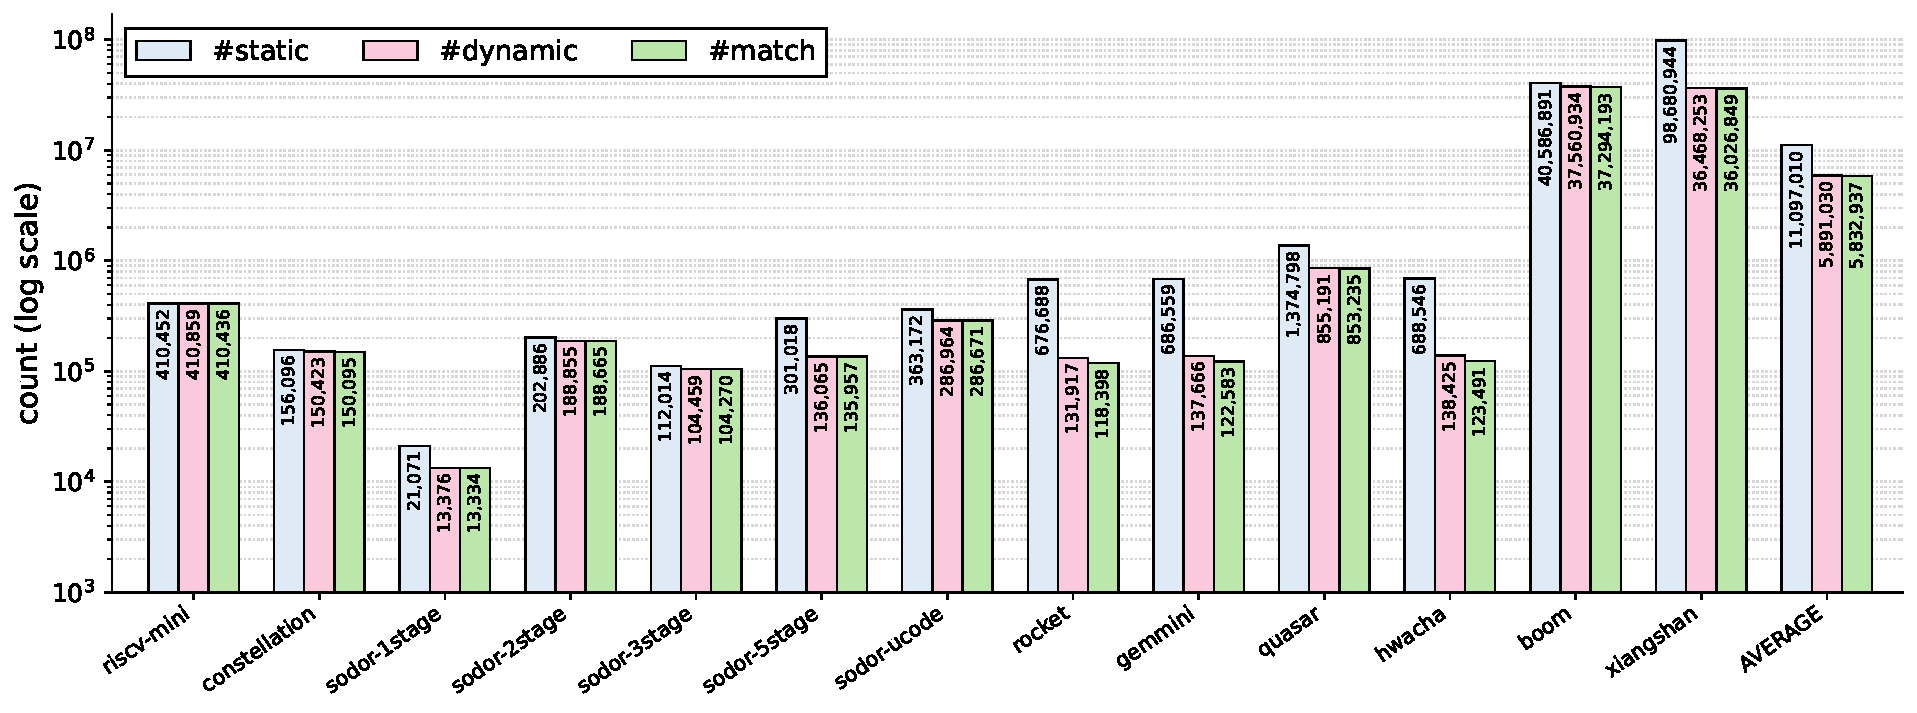
\includegraphics[width=\linewidth,clip,trim=8 10 15 12]{figures/tia-absolute-bars}
    \caption{\tia's results in revealing temporal influence relations in real-world Chisel designs.}\label{fig:tia-absolute}
\end{figure}


Figure~\ref{fig:tia-absolute} presents \tia's results in revealing temporal influence relations in real-world Chisel designs.
The absolute numbers of temporal influence relations captured by \tia (\texttt{\#static}), by runtime instrumentation (\texttt{\#dynamic}), and by both (\texttt{\#match}) are labeled on each bar.
The recall and precision calculated from the statistics in Figure~\ref{fig:tia-absolute} using Equation~\ref{eq:recall-precision} are presented in Figure~\ref{fig:tia-percent}.
Figure~\ref{fig:tia-percent} also presents the analysis time for each benchmark in the parentheses under the bars as an indication of \tia's efficiency.
Below, we separately detail \tia's soundness, precision, and efficiency based on these empirical results.

\begin{figure}[tp]
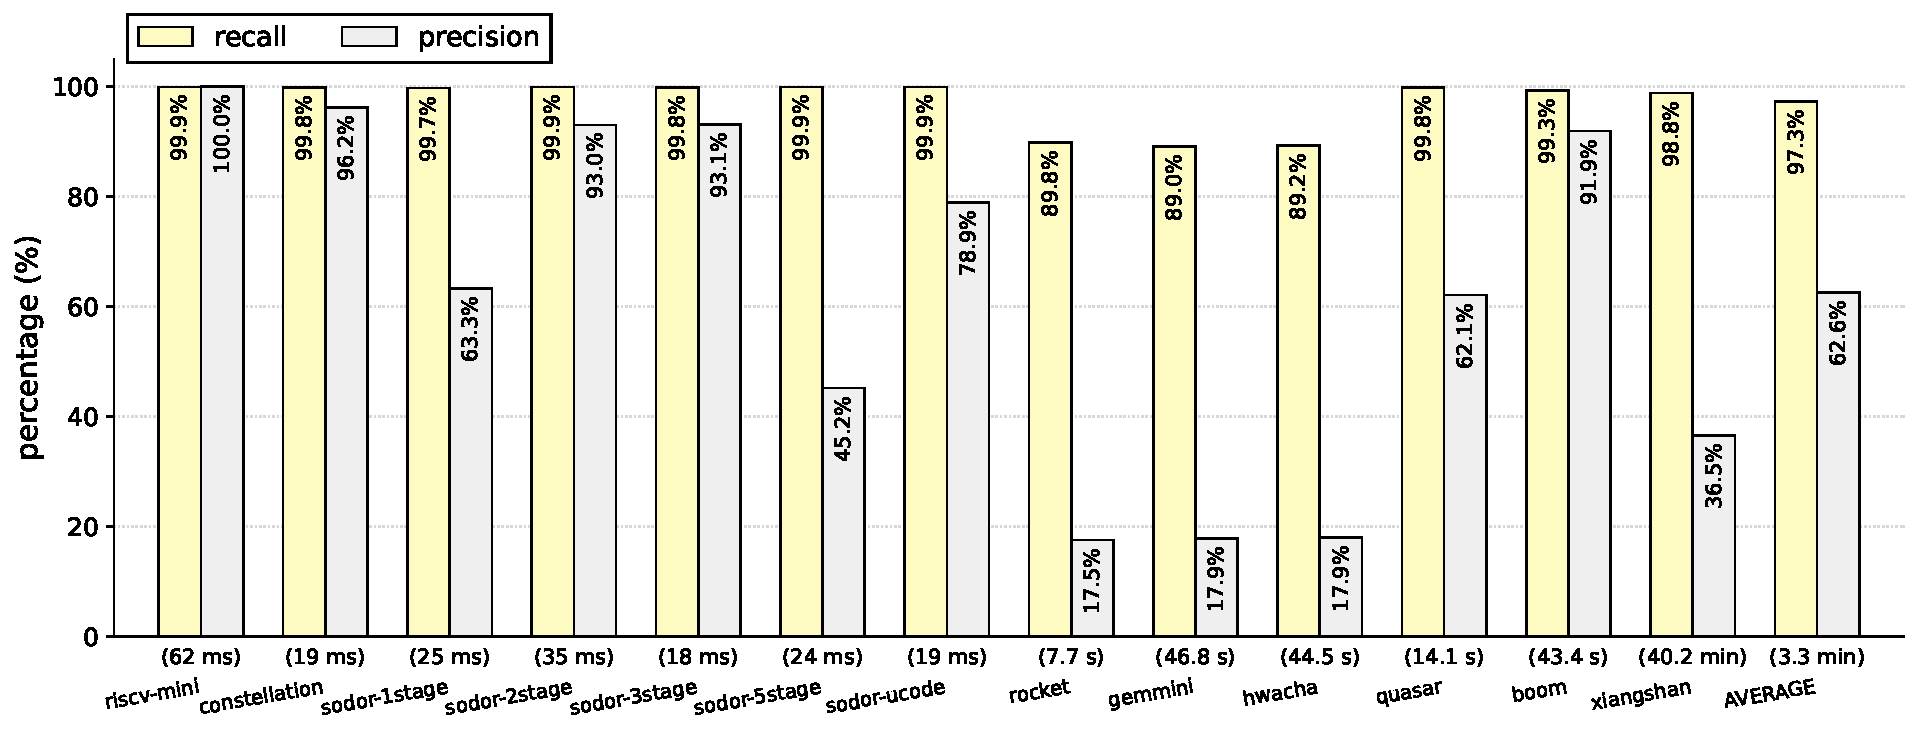
\includegraphics[width=\linewidth,clip,trim=8 9 18 5]{figures/tia-percent-bars}
\caption{Effectiveness of \tia on real-world Chisel designs, including recall (yellow bars), precision (gray bars), and efficiency (analysis time shown in parentheses under each bar).}\label{fig:tia-percent}
\end{figure}

\paragraph{Soundness}

\tia demonstrates strong empirical soundness, achieving an average recall of 97.3\%, as shown in the last column of Figure~\ref{fig:tia-percent}.
This high recall provides empirical evidence consistent with \tia's theoretical soundness. % TODO: in Theorems~\ref{theo:soundness} and~\ref{theo:}.
The small recall loss arises primarily from two limitations in handling complex real-world hardware designs.
(1) For external hardware modules whose source code is written in Verilog rather than Chisel, we model them as black boxes and assume a one-cycle delay between any input and output port.
This treatment is currently a heuristic engineering choice;
for example, the \texttt{plusarg\_reader} module in \texttt{rocket} cannot be soundly modeled using this heuristic.
Future work could investigate more systematic approaches, such as interactive static analysis across Chisel and Verilog.
(2) Since \tia's current theory focuses on synchronous hardware with a single global clock, for multiple-clock designs such as \texttt{hwacha} and \texttt{gemmini}, our implementation applies \tia rules independently to each clock domain as an engineering approximation.
This treatment may miss subtle temporal behaviors involving clock-domain crossings (CDCs)~\cite{chong_clock_2021}.
Future work could extend \tia's theory to multi-clock designs by explicitly tracking temporal influences with respect to each clock and developing rules for temporal interactions across clock domains.

\paragraph{Precision}
As the first static analysis primarily designed to soundly reason about infinite temporal influences in hardware designs, \tia achieves reasonable precision, with an average precision of 62.6\%, as shown in the last column of Figure~\ref{fig:tia-percent}.
This measured precision is an under-estimation of \tia's actual precision because we evaluate against only a subset of the true ground truth obtained through runtime instrumentation;
temporal influences reported by \tia but not observed dynamically may correspond to true influences that were simply not exercised during simulation.
Beyond this inherent under-estimation, we observe two major sources of imprecision in \tia.
\emph{(1) Memory Cell Insensitivity.}
For efficiency, we currently abstract an entire memory as a single abstract memory cell when analyzing memory accesses.
This coarse-grained abstraction can merge distinct temporal influence flows when they propagate through the memory, introducing false positives.
For example, the largest Chisel memory in \texttt{rocket} contains 16,384 cells, all of which are merged into a single abstract memory cell.
Although this abstraction is sound, it can introduce substantial imprecision.
A finer-grained memory abstraction could alleviate this problem and constitutes a direction for future work.
\emph{(2) Path Insensitivity.}
We currently soundly assume that the condition of each multiplexer (analogous to an \texttt{if}-statement in software) can evaluate to either true or false.
This path-insensitive treatment can introduce false positives.
For example, the conditions $a$ and $\neg a$ cannot both be true or both be false simultaneously, but our current analysis cannot exploit this mutual exclusivity to eliminate the corresponding false positives.
Introducing path sensitivity in the future could therefore further improve \tia's precision.


\paragraph{Efficiency}

As shown in Figure~\ref{fig:tia-percent}, \tia analyzes the 13 real-world hardware designs, totaling 5.9M LoC, in 42.8 minutes in total, 510.7$\times$ faster the 364.3 hours required by dynamic runtime instrumentation while achieving an average recall of 97.3\% in capturing dynamically observed temporal influences.
This result demonstrates the efficiency advantage of static analysis over simulation-based approaches for analyzing real-world hardware designs containing millions of lines of code.
The slowest case is \texttt{xiangshan}, which takes 40.2 minutes to analyze due to its large size of 4.0M LoC, yet remains substantially more efficient than dynamic simulation.


\subsection{RQ2: Potential of \tia to Support Diverse Hardware Analysis Clients}

To demonstrate the potential of \tia to support diverse hardware analysis clients, we develop three client analyses on top of \tia:
a hardware bug detection client---signal asynchrony analysis (Section~\ref{sec:client-asynchrony}),
a hardware security analysis client---timing-flow analysis (Section~\ref{sec:client-timingflow}),
and a hardware design understanding client---timeline interface analysis (Section~\ref{sec:client-timeline}).
We evaluate the three clients on their respective tasks to provide empirical evidence of \tia's practical potential.

\subsubsection{Hardware Bug Detection: Signal Asynchrony Analysis}\label{sec:eval-asynchrony}

The signal asynchrony analysis is described in Section~\ref{sec:client-asynchrony};
this section focuses on its evaluation (Figure~\ref{fig:eval-asynchrony}).

\begin{figure}[tp]
    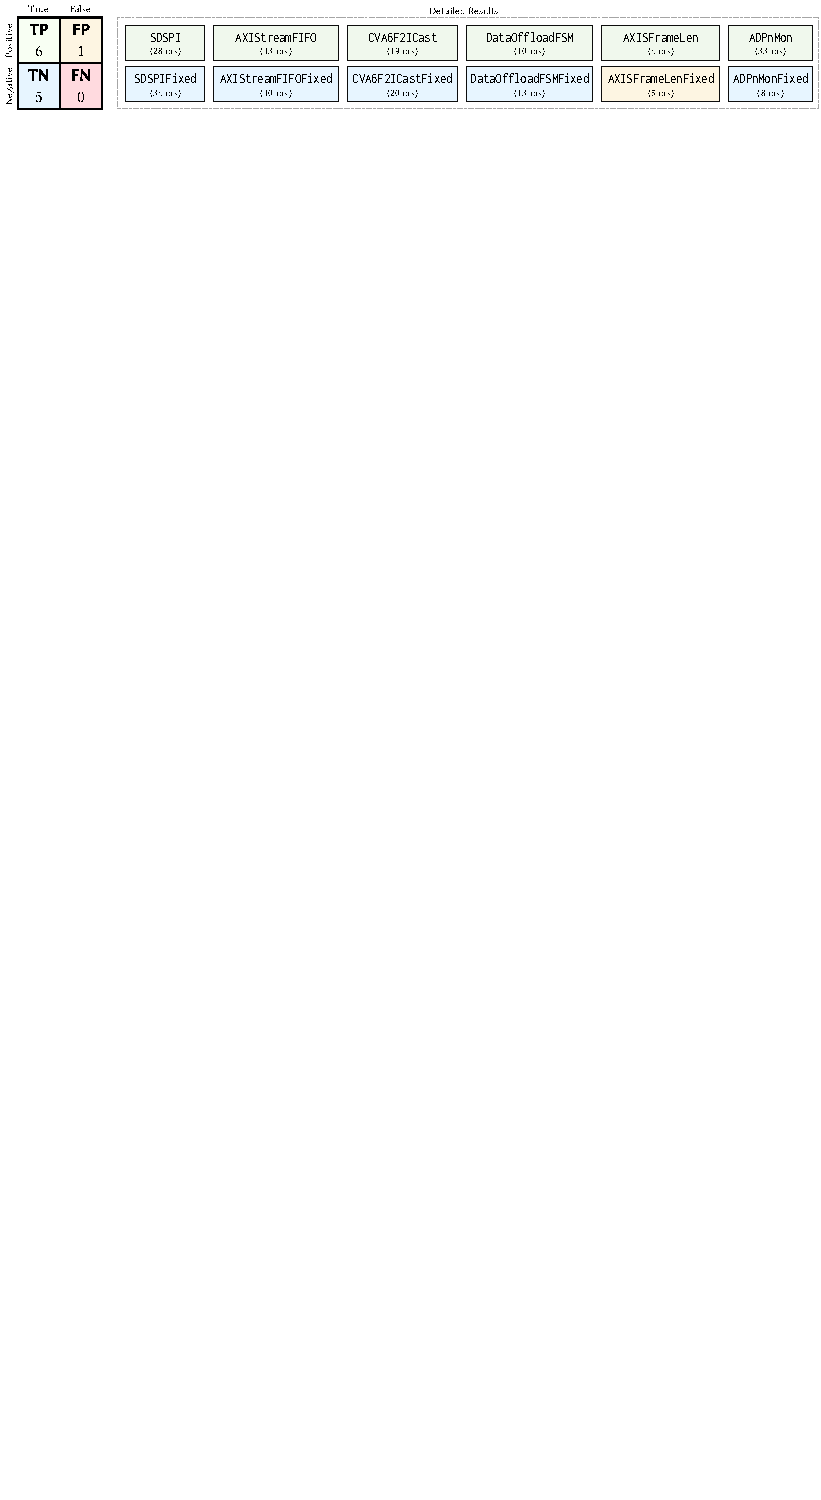
\includegraphics[clip,trim=0 23.5cm 0 0]{figures/asynchrony-eval}
    \caption{Evaluation of signal asynchrony analysis (recall: 100\%, precision: 85.7\%), a hardware bug detection client built on top of \tia; analysis times are shown in parentheses.}\label{fig:eval-asynchrony}
\end{figure}

\paragraph{Benchmarks}
Our signal asynchrony analysis is inspired by a survey of hardware bugs~\cite{ma_debugging_2022}, which defines signal asynchrony bugs and reproduces two such bugs from bug-fixing commits in open-source hardware projects: an SD card controller (\texttt{SDSPI}~\cite{sdspi}) and an AXI4-stream FIFO (\texttt{AXIStreamFIFO}~\cite{axi-stream-fifo}).
We use both the buggy and corresponding fixed versions of these two designs as benchmarks, yielding four benchmarks in the dashed box in Figure~\ref{fig:eval-asynchrony};
the fixed versions are denoted by appending the \texttt{Fixed} suffix to their original names.

The artifact~\cite{ma_debugging_2022_artifact} accompanying the survey~\cite{ma_debugging_2022} additionally lists eight signal asynchrony bug-fixing commits but does not provide proof-of-concept tests to reproduce their buggy behavior.
We attempted to reproduce these bugs and successfully developed proof-of-concept tests for four of them:
a floating-point unit (FPU) component (\texttt{CVA6F2ICast}~\cite{cva6-f2i-cast}),
a storage unit access controller (\texttt{DaraOffloadFSM}~\cite{data-offload-fsm}),
a network interface controller component for frame monitoring (\texttt{AXISFrameLen}~\cite{axis-frame-len}), and
a pseudo-random number monitor (\texttt{ADPnMon}~\cite{ad-pn-mon}).
Together with their corresponding fixed versions, these four buggy designs yield eight additional benchmarks, also shown in the dashed box in Figure~\ref{fig:eval-asynchrony}.

For the remaining four bug-fixing commits listed in the artifact~\cite{ma_debugging_2022_artifact}, our investigation found that three are outside the scope of the signal asynchrony bugs defined by the survey.
The remaining commit modifies 68 files, and we could not identify a reproducible signal asynchrony bug from it.

\paragraph{Understanding the Results}
The left part of Figure~\ref{fig:eval-asynchrony} summarizes the overall results of signal asynchrony analysis, while the right part details the results for each benchmark, with colors indicating the classification.
There are 6 true positives (TPs, in green), where our analysis correctly identifies buggy designs as buggy, and 5 true negatives (TNs, in blue), where it correctly identifies non-buggy designs as non-buggy.
There are no false negatives (FNs, in red), where our analysis fails to detect a true asynchrony bug, yielding a recall of $\mathit{recall} = \mathit{TP}/(\mathit{TP}+\mathit{FN}) = 100\%$.
There is only one false positive (FP, in yellow), where our analysis reports a asynchrony bug in a non-buggy design, yielding a precision of $\mathit{precision} = \mathit{TP}/(\mathit{TP}+\mathit{FP}) = 85.7\%$.

The false positive occurs in \texttt{AXISFrameLenFixed}.
This module expects its AXI monitor interface inputs to follow a specific protocol, under which its outputs \texttt{frameLen} and \texttt{frameLenValid} are synchronized by the input \texttt{monitorAxisTlast}.
However, our analysis does not incorporate this input constraint and therefore considers these outputs potentially asynchronous under unconstrained inputs.
Thus, although the bug is fixed under the module's intended input protocol, our analysis reports a potential asynchrony under unconstrained inputs, resulting in the false positive.

As indicated by the analysis times in parentheses under the benchmark names in Figure~\ref{fig:eval-asynchrony}, our signal asynchrony analysis is also efficient, taking an average of 16.4 milliseconds across the benchmarks, including the time spent by the underlying \tia.
This efficiency stems from both the efficiency of \tia and the lightweight reuse of its computed temporal influence information: the client analysis only queries \tia's results to check signal synchronization, as described in Section~\ref{sec:client-asynchrony}, and therefore incurs little additional computational overhead.

\subsubsection{Hardware Security Analysis: Timing-flow Analysis}

The timing-flow analysis is described in Section~\ref{sec:client-timingflow};
this section focuses on its evaluation (Figure~\ref{fig:eval-timingflow}).

\begin{figure}[tp]
    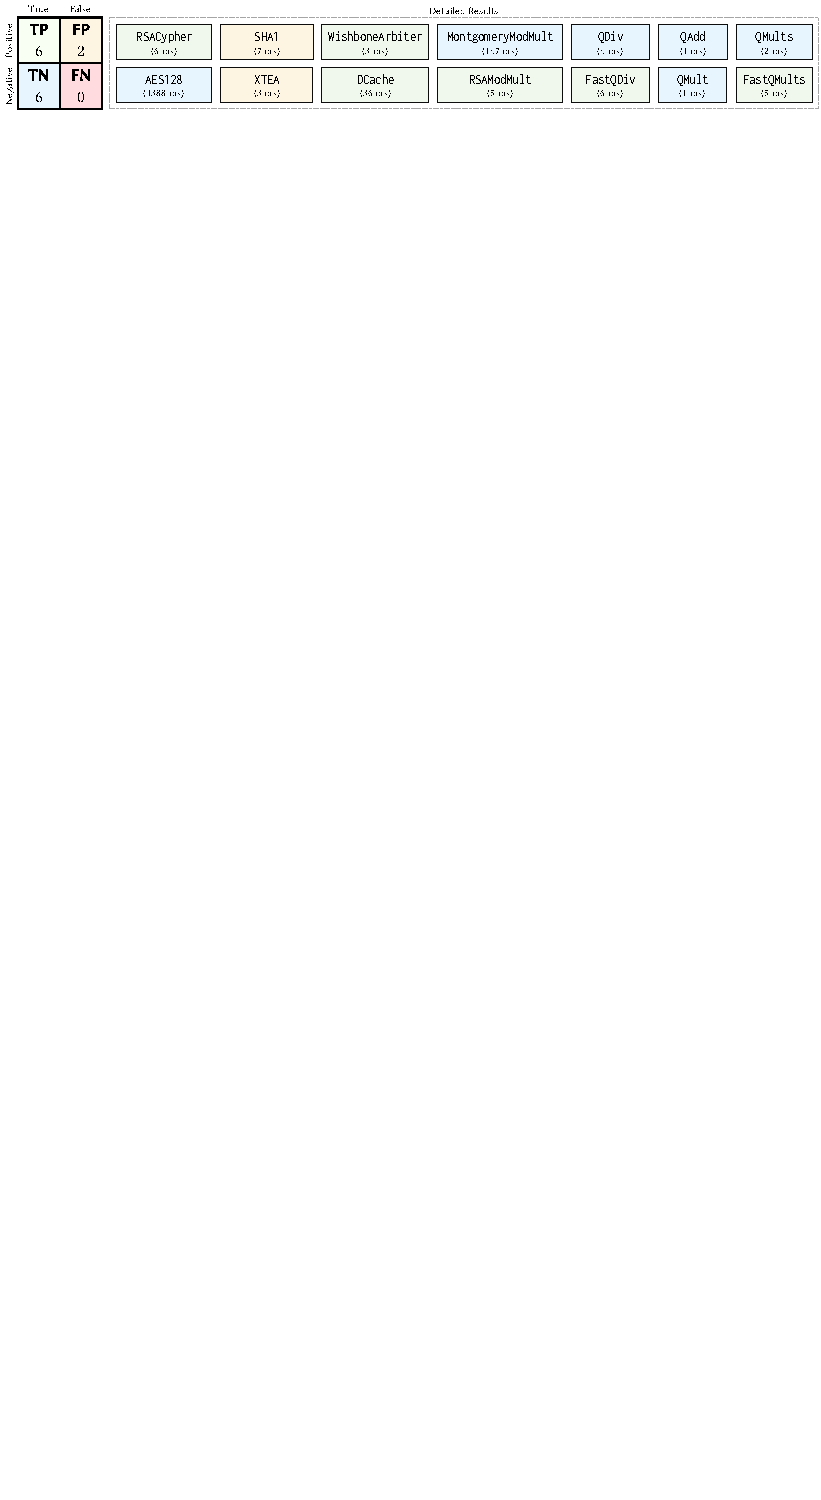
\includegraphics[clip,trim=0 23.5cm 0 0]{figures/timingflow-eval}
    \caption{Evaluation of timing-flow analysis (recall: 100\%, precision: 75\%), a hardware security client built on top of \tia; analysis times are shown in parentheses.}\label{fig:eval-timingflow}
\end{figure}

\paragraph{Benchmarks}

Our timing-flow analysis is inspired by a survey of hardware information-flow tracking~\cite{hu_hardware_2022}, which describes information leaks through timing flows and summarizes representative hardware designs for which prior work~\cite{ardeshiricham_clepsydra_2017,qin_formal_2020,alatoun_efficient_2022} has established the presence or absence of timing flows.
We select all such designs available to us as benchmarks to evaluate our timing-flow analysis.
These designs, shown in the dashed box in the right part of Figure~\ref{fig:eval-timingflow}, include cryptographic components from TrustHub~\cite{salmani_design_2013,shakya_benchmarking_2017} (\texttt{RSACypher}~\cite{rsa-cypher} and \texttt{AES128}~\cite{aes128}) and OpenCores~\cite{opencores} (\texttt{SHA1}~\cite{sha1} and \texttt{XTEA}~\cite{xtea}), a round-robin-based Wishbone arbiter (\texttt{WishboneArbiter}~\cite{wishbone-arbiter}), a data cache (\texttt{DCache} described by~\cite{qin_formal_2020}), modular multipliers (\texttt{MontgomeryModMult}~\cite{montgomery-modmult} and \texttt{RSAModMult}~\cite{rsa-modmult}), and fixed-point arithmetic units~\cite{fixed-point-math} and their variants described by~\cite{qin_formal_2020,ardeshiricham_clepsydra_2017}.

\paragraph{Understanding the Results}


The left part of Figure~\ref{fig:eval-timingflow} summarizes the overall results of timing-flow analysis, while the right part details the results for each benchmark, with colors indicating the classification.
There are 6 true positives (TPs, in green), where our analysis correctly identifies timing-flow information leaks in vulnerable designs, and 6 true negatives (TNs, in blue), where it correctly identifies secure designs without timing flows as secure.
There are no false negatives (FNs, in red), where our analysis fails to detect a true timing-flow information leak, yielding a recall of $\mathit{recall} = \mathit{TP}/(\mathit{TP}+\mathit{FN}) = 100\%$.
There are two false positives (FPs, in yellow), where our analysis reports a timing-flow information leak in a secure design, yielding a precision of $\mathit{precision} = \mathit{TP}/(\mathit{TP}+\mathit{FP}) = 75\%$.
The two false positives occur in \texttt{SHA1} and \texttt{XTEA} and are caused by \tia's path insensitivity.
Specifically, path insensitivity allows spurious temporal influences from the private source to the public sink that indicate timing flows, even though not all of these influences can occur under the actual combination of multiplexer conditions.

As indicated by the analysis times in parentheses under the benchmark names in Figure~\ref{fig:eval-timingflow}, our timing-flow analysis is also efficient, taking an average analysis time of 115.3 milliseconds across the benchmarks, including the time spent by the underlying \tia.
This efficiency stems from both the efficiency of \tia and the lightweight reuse of its computed temporal influence information: the client analysis only queries \tia's results to identify multiple temporal influences that indicate timing flows, as described in Section~\ref{sec:client-timingflow}, and therefore incurs little additional computational overhead.
The \texttt{AES128} benchmark takes more than one second to analyze, substantially longer than the other benchmarks combined, because it is much larger than the other benchmarks combined (98.4K LoC vs. 1.6K LoC in pre-elaborated Firrtl~\cite{izraelevitz_reusability_2017}).

\subsubsection{Hardware Design Understanding: Timeline Interface Analysis}

The timeline interface analysis is described in Section~\ref{sec:client-timeline};
this section focuses on its evaluation (Figure~\ref{fig:eval-timeline}).

\begin{figure}[tp]
    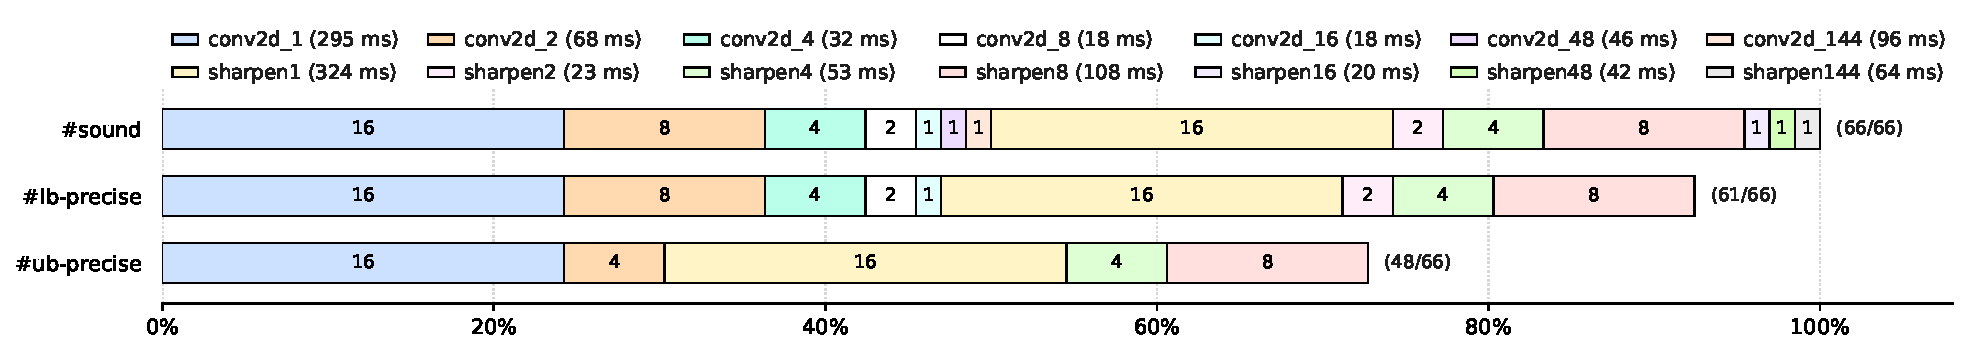
\includegraphics[width=\linewidth,clip,trim=8 9 11 15]{figures/timeline-eval}
    \caption{
        Evaluation of timeline interface analysis (a hardware design understanding client built on top of \tia), where \texttt{\#sound} denotes the number of inferred timeline intervals that are supersets of the corresponding ground-truth intervals (recall: 100\%),
        \texttt{\#lb-precise} denotes the number of inferred timeline intervals with a precise lower bound (lower-bound precision: 92.4\%), and
        \texttt{\#up-precise} denotes the number of inferred intervals with a precise upper bound (upper-bound precision: 72.7\%).
        Analysis times are shown in parentheses.
    }\label{fig:eval-timeline}
\end{figure}

\paragraph{Benchmarks}

Our timeline interface analysis is inspired by the hardware timeline type system~\cite{nigam_modular_2023}, which specifies the clock-cycle intervals during which each input or output is required or available, providing a convenient interface for hardware designers to understand the temporal behavior of a hardware module.
We therefore reuse the hardware designs evaluated in~\cite{nigam_modular_2023}, whose timeline interfaces are established by the type system, as benchmarks for evaluating our timeline interface analysis.
The benchmarks include 14 designs, shown in Figure~\ref{fig:eval-timeline}, implementing two image-processing accelerator kernels (\texttt{conv2d} and \texttt{sharpen}), with 7 design points for each kernel representing different resource-throughput trade-offs.

\paragraph{Understanding the Results}

Figure~\ref{fig:eval-timeline} presents the results of timeline interface analysis.
Across the 66 top-module output ports in the benchmarks, our timeline interface analysis infers 66 timeline intervals with the following results.
\emph{First}, all 66 inferred intervals are sound, i.e., they are supersets of the corresponding ground-truth intervals, yielding a recall of 100\%.
\emph{Second}, 61 inferred intervals have a precise lower bound, yielding a lower-bound precision of $61/66 = 92.4\%$.
\emph{Third}, 48 inferred intervals have a precise upper bound, yielding an upper-bound precision of $48/66 = 72.7\%$.
Thus, the upper-bound precision is lower than the lower-bound precision.

The lower upper-bound precision is primarily caused by imprecision in the underlying \tia, which can introduce false-positive temporal influences at larger, potentially unbounded clock cycles due to widening and path insensitivity.
For example, in \texttt{conv2d\_4}, each output has a ground-truth timeline interval of $[G+6, G+7)$, whereas our timeline interface analysis reports $[G+6, G+9)$.
Although the inferred interval is sound and has a precise lower bound, its upper bound is imprecise because the underlying \tia reports two false-positive temporal influence objects at clock cycles 7 and 8.
In the worst case, the inferred upper bound is infinity, which occurs for 4 of the 66 ports.
For example, the output port $O$ of \texttt{conv2d\_48} has a ground-truth timeline interval of $[G+12, G+13)$, whereas our analysis reports $[G+9, G+\infty)$.
This imprecision arises because path insensitivity in the underlying \tia can introduce a loop in the temporal influence graph (TIG), causing infinitely many temporal influences to propagate to $O$ and resulting in an infinite upper bound, as described in Section~\ref{sec:client-timeline}.
We think improving the precision of \tia in future work could improve the precision of this hardware design understanding client.

As indicated by the analysis times in parentheses to the right of the benchmark names in Figure~\ref{fig:eval-timeline}, our timeline interface analysis is efficient, taking an average analysis time of 86.2 milliseconds across the benchmarks, including the time spent by the underlying \tia.
This efficiency stems from both the efficiency of \tia and the lightweight reuse of its computed temporal influence information: the client analysis only queries \tia's results to compute the minimal interval containing all clock cycles occurring in the temporal influence objects, as described in Section~\ref{sec:client-timeline}, and therefore incurs little additional computational overhead.






\section{Related Work}

Recent work has increasingly invested effort in applying programming language techniques to hardware description languages (HDLs)~\cite{truong_golden_2019,chen_essence_2023,schuiki_llhd_2020,loow_simulation_2025,nigam_modular_2023,christensen_wire_2021,bourgeat_making_2025,jang_modular_2024,sisco_loop_2023,zagieboylo_pdl_2022,bourgeat_essence_2020,vega_reticle_2021,koeplinger_spatial_2018,durst_type-directed_2020,pelton_wavefront_2024,choi_revamping_2025,malik_circuit_2025,chen_allo_2024,nigam_predictable_2020,lee_optimizing_2020,herklotz_hyperblock_2024,law_mechanized_2025,kim_unifying_2024,fehr_first-class_2025,cui_chisa_2026,yan_verieq_2026,chen_exploiting_2026,kong_improving_2026}.
Our work on advancing static analysis for Chisel~\cite{bachrach_chisel_2012,izraelevitz_reusability_2017}---the most popular modern HDL---is part of this broader effort.
This section first reviews the most relevant prior work on static analysis for HDLs and then discusses other related work.

\paragraph{Static Analysis for HDLs}


\paragraph{Formal Verification for Chisel}


\paragraph{Detecting Signal Asynchrony Bugs}

just a survey, provides some instrumenting methods

\paragraph{Identifying Timing Flows}

information flow tracking

\paragraph{Understanding Timeline Interfaces}

type systems


\input{conc}

\bibliographystyle{ACM-Reference-Format}
\bibliography{references}

\end{document}
